\chapter{zTikZ{}宏包}
目前zTikZ宏包能够在Linux下编译运行,在Windows上还未进行完整的测试. 但是对于\TeX{}Live版本 $\ge$2023的
用户来说,本宏包应该是可以在Linux和Windows下运行的. 实际的兼容情况应该得等到足够的用户反馈时才能够确定.

\section{基本介绍}
\subsection{zTikZ{}功能}
zTikZ宏包主要用于绘图与计算, 其中的绘图功能支持\cmd{python, mathematica, gnuplot}, 但是
这并不意味着你需要安装以上给的所有软件,每一个软件(模块)之间是独立的。当你需要什么功能的时候
再去在操作系统上安装对应的模块即可.

zTikZ主要提供两个大功能: \textbf{绘图, 计算}.
绘图部分包括TikZ自身的绘图功能(2d部分)\Footnote{由于3d绘图部分涉及的几个变换矩阵我还没想好怎么融合进入TikZ, 
所以目前ZTikZ不提供3d绘图功能},python的matplotlib绘图,以及mathematica代码绘图. 计算部分
包括\LaTeX3的\cmd{xfp}宏包模块,python的sympy计算模块,以及mathematica计算. 

\subsection{缓存机制}
zTikZ除了提供必要的和外部程序互动的功能外,还内置了一套cache系统,zTikZ会自动把\TeX{}和
外部程序交互产生的结果保存下来,记录下\LaTeX{}文档中调用的源代码的Hash值,如果\LaTeX{}文档中的源代码
Hash值改变,那么ZTikZ就会重新和外部程序交互,重新产生结果,并且缓存新的Hash值。如果文档中的
源代码的Hash值没有变,那么ZTikZ就会直接调用上一次的缓存结果. 这样做的好处是显而易见的,就是
我们不必反复的编译没有变化的内容,直接引用缓存,大大的减少了编译的时间. 

目前zTikZ中的所有模块:TikZ/gnuplot\Footnote{\cmd{tikzpicture}环境或者是\cmd{\tikz}命令生成图片的cache机制是依靠
tikz的\cmd{external}库实现的,感兴趣的可以去看看}, Python/sympy, Python/matplotlib, Mathematica都已经实现
了缓存机制. 在实际测试中,第一次编译耗时 1min10s左右,但是在结果缓存后,再次编译源文档便只需要3s就可以
结束. 每一个部分的源代码被修改后,对应的部分都会重新计算,重新生成结果,并记录下新的Hash值为下一次的
缓存做准备。

目前zTikZ可以在加载宏包时指定是否开启\cmd{tikzpicture}环境的缓存机制,如果你不想使用缓存机制,那么可以
使用如下格式加载宏包(zTikZ默认缓存所有环境内容):
\begin{codeprint}
\usepackage[external=false]{ztikz}
\end{codeprint}

\section{Set Up zTikZ}
\subsection{兼容情况}
目前\cmd{zTikZ}模块已经可以做到跨平台, 在各个平台中的兼容性如下:

\hspace*{10em}\parbox{8cm}{
\begin{itemize}
    \item[Windows]: \TeX{}Live最低版本2023
    \item[Linux]: \TeX{}Live最低版本2022
    \item[MacOS]: Mac\TeX{}由于缺少\cmd{l3sys-shell}宏包(或者是不适配),所以并不兼容
\end{itemize}}

在Linux平台上并没有什么需要注意的事项,重点是Windows平台上的兼容性; 使用\cmd{zTikZ}正常运行,
那么在你的系统中(默认添加了环境变量)须有以下软件:
\begin{itemize}
    \item \cmd{gnuplot}: zTikZ库的二维绘图功能均基于gnuplot,所以你需要在你的本地安装gnuplot.
    \item \cmd{python}: 用于运行python脚本进行符号计算与绘图,需要Python库\cmd{sympy, scipy}.
    \item \cmd{sed}: 主要用于绘图脚本中的函数以及绘制样式替换,后续可能会考虑去除\cmd{sed}依赖.
    \item \cmd{wolframscript}(可选):如果需要使用本模块的Mathematica功能,那么需要安装WolframScript以及
        对应的Mathematica软件.或者只安装wolframscript,但是在执行命令时选择在云端执行,这样就不用
        本地的Mathematica计算内核了. 
\end{itemize}

\subsection{环境配置}
\subsubsection{Linux}
在Linux下除了wolfram应该都是很好安装的, 直接使用Linux发行版自带的包管理器即可.在这里我提供一个在
WSL中使用Windows下Mathematica 的方法. 其实就是在Linux下创建一个从Linux到Windows的软连接,如下:

\begin{codeprint}
ln -sf "/mnt/c/Program Files/Wolfram Research/WolframScript/wolframscript.exe" /usr/bin/wolframscript    
\end{codeprint}

具体的wolframscript的路径根据实际情况而定.

\subsubsection{Windows}
由于目前我的Windows环境中的\TeX{}Live版本过低,无法测试相关的功能,所以目前zTiKZ在Windows下
是出于搁置状态的\Footnote{但是zTiKZ中的Wolfram模块是可以在Windwos上使用的,这一点弥补了 
\href{https://github.com/stevenliuyi/latex-alpha2}{latexalpha2} 的不足}.
也许等一段时间,在我装上\TeX{}Live 2024后,我也许会试一试zTikZ模块的跨平台兼容性.

因会使用到\cmd{gnuplot},所以在Windows下需要在系统环境变量中添加\cmd{gnuplot}的路径.并且
在编译此文档时需要加上对应的 \cmd{--shell-esape}参数;在Windows平台,由于\TeX{}Live的编译配置,
需确保系统环境变量\cmd{PATHEXT}中已经删除\cmd{.PY}后缀. zTiKZ在Windows下的适配是没有Linux下那么好的,
建议在Linux下使用本宏包.\Footnote{但是zTiKZ中的Wolfram模块是可以在Windwos上使用的,这一点弥补了 
\href{https://github.com/stevenliuyi/latex-alpha2}{latexalpha2} 的不足}.

\section{绘图功能}
\subsection{tikz/gnuplot}
zTikZ提供了绘制绝大部分函数的命令,同时zTikZ的命令可以和\cmd{tikz}中的命令``融合'',它们
可以在同一个\cmd{tikzpicture}环境中使用. 而且,zTikZ对函数绘制时的坐标进行了``对齐''. 
也就是zTikZ中命令的坐标,和\cmd{TiKZ}中的命令的坐标, Geogebra中的坐标是一致的. 为何要在
zTiKZ中把坐标``对齐''? 试想这么一个情景:你在Geogebra中找到了两个函数图像的交点为 $P(1, 2)$,
你首先使用TiKZ自带的\cmd{\filldraw}命令把这个 $P$点绘制出来了, 但是然后你使用zTikZ中的
\cmd{\ShowPoint}命令也是绘制这个 $P$点,但是这两个 $P$点却没有重合,尽管我们指定的坐标
都是 $(1, 2)$. 这就是为什么zTikZ要把坐标``对齐''. 这样还有一个好处,当你不方便使用 zTikZ 
求解某些特殊的点时,你可以在Geobebra把 $P$点求解出来,然后直接在zTikZ中使用\cmd{\ShowPoint}命令
把这个点绘制出来, 不用担心它们没有对齐.

在平面图形绘制方面,zTikZ提供了绘制函数命令,一些和坐标轴有关的命令以及部分的欧几里得几何相关的命令,
各命令\Footnote{zTiKZ中的命令基本上都遵守了Mathematica中的函数的命名规范}的名称如下:

\begin{multicols}{2}
\begin{itemize}
    \item 函数绘制
        \begin{itemize}
            \item \cmd{\Plot}\index{\cmd{\Plot}}: 绘制函数
            \item \cmd{\ParamPlot}\index{\cmd{\ParamPlot}}: 绘制参数方程
            \item \cmd{\ContourPlot}\index{\cmd{\ContourPlot}}: 绘制等高线图
            \item \cmd{\PolarPlot}\index{\cmd{\PolarPlot}}: 绘制极坐标图
            \item \cmd{\ListPlot}\index{\cmd{\ListPlot}}: 绘制散点图,只需要指定绘制参数中\cmd{opacity=0}
            \item \cmd{\StairsPlot}\index{\cmd{\StairsPlot}}: 绘制阶梯图
            \item \cmd{\StemPlot}\index{\cmd{\StemPlot}}: 绘制火柴棒图
            \item \cmd{\BarPlot}\index{\cmd{\BarPlot}}: 绘制条形图
            \item \cmd{\ShadePlot}\index{\cmd{\ShadePlot}}: 绘制渐变曲线(直线)
            \item \cmd{\PlotPrecise}\index{\cmd{\PlotPrecise}}: 函数绘制精度
        \end{itemize}
    \item 欧几里得几何 
        \begin{itemize}
            \item \cmd{\ShowPoint}\index{\cmd{\ShowPoint}}: 绘制点
            \item \cmd{\Polygon}\index{\cmd{\Polygon}}: 绘制正多边形
            \item \cmd{\ShowGrid}\index{\cmd{\ShowGrid}}: 绘制网格 
            \item \cmd{\ShowAxis}\index{\cmd{\ShowAxis}}: 绘制坐标轴
            \item \cmd{\ShowIntersection}\index{\cmd{\ShowIntersection}}: 绘制交点
            \item \cmd{\gnudata}\index{\cmd{\gnudata}}:引用gnuplot数据
        \end{itemize}
\end{itemize}
\end{multicols}

\begin{remark}
    上述的\cmd{\StairsPlot, \StemPlot, \BarPlot, \ShadePlot}在绘制时只能够传入具体的数据文件,而非
    对应的方程.
\end{remark}

\subsection{Support Functions}
在开始介绍之前,我想介绍一下gnuplot中支持的函数,见\cref{tab:gnuplot-functions},
摘录自\href{http://www.bersch.net/gnuplot-doc/expressions.html#expressions-functions-floor}{gnuplot-support-functions}:

\begin{leftbar}
    Arguments to math functions in gnuplot can be integer, real, or complex unless otherwise noted.
    Functions that accept or return angles (e.g. sin(x)) treat angle values as radians, but this may 
    be changed to degrees using the command set angles.
\end{leftbar}

\begin{center}
    \begin{longtable}{lll}
        \caption{\textbf{Math library functions}}\\
        \toprule
        \textbf{Function} & \textbf{Arguments} & \textbf{Returns} \\
        \midrule
        \(\text{abs}(x)\) & any & $|x|$, absolute value of $x$; same type \\
        \(\text{abs}(x)\) & complex & length of $x$, $\sqrt{\text{Re}(x)^2 + \text{Im}(x)^2}$ \\
        \(\text{acos}(x)\) & any & $\cos^{-1} x$ (inverse cosine) \\
        \(\text{acosh}(x)\) & any & $\cosh^{-1} x$ (inverse hyperbolic cosine) in radians \\
        \(\text{airy}(x)\) & any & Airy function $\text{Ai}(x)$ \\
        \(\text{arg}(x)\) & complex & the phase of $x$ \\
        \(\text{asin}(x)\) & any & $\sin^{-1} x$ (inverse sine) \\
        \(\text{asinh}(x)\) & any & $\sinh^{-1} x$ (inverse hyperbolic sine) in radians \\
        \(\text{atan}(x)\) & any & $\tan^{-1} x$ (inverse tangent) \\
        \(\text{atan2}(y,x)\) & int or real & $\tan^{-1}(y/x)$ (inverse tangent) \\
        \(\text{atanh}(x)\) & any & $\tanh^{-1} x$ (inverse hyperbolic tangent) in radians \\
        \(\text{EllipticK}(k)\) & real  $k$ in $(-1:1)$ & $K(k)$ complete elliptic integral of the first kind \\
        \(\text{EllipticE}(k)\) & real  $k$ in $[-1:1]$ & $E(k)$ complete elliptic integral of the second kind \\
        \(\text{EllipticPi}(n,k)\) & real $n<1$, $k$ in $(-1:1)$ & $\Pi(n,k)$ complete elliptic integral of the third kind \\
        \(\text{besj0}(x)\) & int or real & $J_0$ Bessel function of $x$, in radians \\
        \(\text{besj1}(x)\) & int or real & $J_1$ Bessel function of $x$, in radians \\
        \(\text{besy0}(x)\) & int or real & $Y_0$ Bessel function of $x$, in radians \\
        \(\text{besy1}(x)\) & int or real & $Y_1$ Bessel function of $x$, in radians \\
        \(\text{ceil}(x)\) & any & $\lceil x \rceil$, smallest integer not less than $x$ (real part) \\
        \(\text{cos}(x)\) & radians & $\cos x$, cosine of $x$ \\
        \(\text{cosh}(x)\) & any & $\cosh x$, hyperbolic cosine of $x$ in radians \\
        \(\text{erf}(x)\) & any & $\text{erf}(\text{Re}(x))$, error function of $\text{Re}(x)$ \\
        \(\text{erfc}(x)\) & any & $\text{erfc}(\text{Re}(x))$, $1.0 - $ error function of $\text{Re}(x)$ \\
        \(\text{exp}(x)\) & any & $e^x$, exponential function of $x$ \\
        \(\text{expint}(n,x)\) & any & $E_n(x)$, exponential integral function of $x$ \\
        \(\text{floor}(x)\) & any & $\lfloor x \rfloor$, largest integer not greater than $x$ (real part) \\
        \(\text{gamma}(x)\) & any & $\Gamma(\text{Re}(x))$, gamma function of $\text{Re}(x)$ \\
        \(\text{ibeta}(p,q,x)\) & any & $\text{ibeta}(\text{Re}(p,q,x))$, ibeta function of $\text{Re}(p,q,x)$ \\
        \(\text{inverf}(x)\) & any & inverse error function $\text{Re}(x)$ \\
        \(\text{igamma}(a,x)\) & any & $\text{igamma}(\text{Re}(a,x))$, igamma function of $\text{Re}(a,x)$ \\
        \(\text{imag}(x)\) & complex & $\text{Im}(x)$, imaginary part of $x$ as a real number \\
        \(\text{invnorm}(x)\) & any & inverse normal distribution function $\text{Re}(x)$ \\
        \(\text{int}(x)\) & real & integer part of $x$, truncated toward zero \\
        \(\text{lambertw}(x)\) & real & Lambert $W$ function \\
        \(\text{lgamma}(x)\) & any & $\text{lgamma}(\text{Re}(x))$, lgamma function of $\text{Re}(x)$ \\
        \(\text{log}(x)\) & any & $\ln x$, natural logarithm (base $e$) of $x$ \\
        \(\text{log10}(x)\) & any & $\log_{10} x$, logarithm (base 10) of $x$ \\
        \(\text{norm}(x)\) & any & $\text{norm}(x)$, normal distribution function of $\text{Re}(x)$ \\
        \(\text{rand}(x)\) & int & pseudo random number in the interval $(0:1)$ \\
        \(\text{real}(x)\) & any & $\text{Re}(x)$, real part of $x$ \\
        \(\text{sgn}(x)\) & any & $1$ if $x > 0$, $-1$ if $x < 0$, $0$ if $x = 0$. $\Im(x)$ ignored \\
        \(\text{sin}(x)\) & any & $\sin x$, sine of $x$ \\
        \(\text{sinh}(x)\) & any & $\sinh x$, hyperbolic sine of $x$ in radians \\
        \(\text{sqrt}(x)\) & any & $\sqrt{x}$, square root of $x$ \\
        \(\text{tan}(x)\) & any & $\tan x$, tangent of $x$ \\
        \(\text{tanh}(x)\) & any & $\tanh x$, hyperbolic tangent of $x$ in radians \\
        \(\text{voigt}(x,y)\) & real & convolution of Gaussian and Lorentzian \\
        \(\text{cerf}(z)\) & complex & complex error function \\
        \(\text{cdawson}(z)\) & complex & complex Dawson's integral \\
        \(\text{faddeeva}(z)\) & complex & $w(z) = \exp(-z^2) \times \text{erfc}(-iz)$ \\
        \(\text{erfi}(x)\) & real & imaginary error function $\text{erfi}(x) = -i \times \text{erf}(ix)$ \\
        \(\text{VP}(x,\sigma,\gamma)\) & real & Voigt profile \\
        \bottomrule 
        \label{tab:gnuplot-functions}\\
    \end{longtable}
\end{center}
\vspace*{-4em}

\begin{remark}
    \(\text{faddeeva}(z)\): rescaled complex error function
\end{remark}

\subsection{Intruduction to Plot}
我们首先来介绍上面和函数绘制相关的命令,因为它们的参数结构几乎都是一摸一样的, 无论是参数的含义(定义域-样式-函数),
对应参数的位置(均为\cmd{{OOm}}形式的参数). 下面以\cmd{\Plot}命令为例, 讲解这一系列Plot命令的参数格式以及用法:
\begin{codeprint}
\Plot[<plot domain>][<plot style>][<marker options>]{<function>}
\end{codeprint}

其中\cmd{<plot domain>}就是绘制的定义域,比如\cmd{-3:4}; \cmd{<plot style>}为绘制函数的样式,
包括图形的颜色,线型,粗细等等;\cmd{<marker option>}表示是否绘制散点图(意味着此时你要把对应绘制命令的精度降低,
不然会十分的耗时,或者是造成结果的不满意);当你没有指定这个可选参数的值时,默认绘制连续函数的图像.marker 参数采用键值对的 
方式进行指定,见后文\cmd{\ShowPoint}中的\cmd{<marker option>}\index{\cmd{<marker option>}}参数详细解释,二者用法完全一致.
\cmd{<function>}就是你要绘制的函数,比如\cmd{sin(x)}. 以下为一个具体的例子,首先创建一个\cmd{tikzpicture}环境,
在其中写上我们的\cmd{\Plot}命令和对应的绘制参数.

\begin{codeprint}
\begin{tikzpicture}
    \Plot[-1.5*pi:2*pi]{sin(x)}
\end{tikzpicture}
\end{codeprint}

假如你是在命令行编译文档,那么你会看到如下的日志输出:

\begin{codeprint}
\write18 enabled.
entering extended mode
\end{codeprint}

编译结束后,你会得到这样的一个函数图形\Footnote{自然目前这个效果我们是不满意的,
没有坐标轴,网格,刻度等元素.后面我们会慢慢补充这幅图}. 

\begin{center}
    \begin{tikzpicture}
        \Plot[-1.5*pi:pi]{sin(x)}
    \end{tikzpicture}
\end{center}

同时在你的项目文件夹下会生成一个名为\cmd{ztikz_output}的文件夹,这个文件夹在你
第一次运行\cmd{\usepackage{zTikZ}}便会产生,这个文件夹用于存放zTikZ的缓存文件;
现在我们来说说这个文件夹的结构, 当你运行了上面的\cmd{\Plot}命令之后,此文件夹的
结构如下(此时会在\cmd{tikz_data}目录下生成了如\cref{fig:zTikZ-directory}中所示的4个文件):

\begin{figure}[!htb]
    \centering
    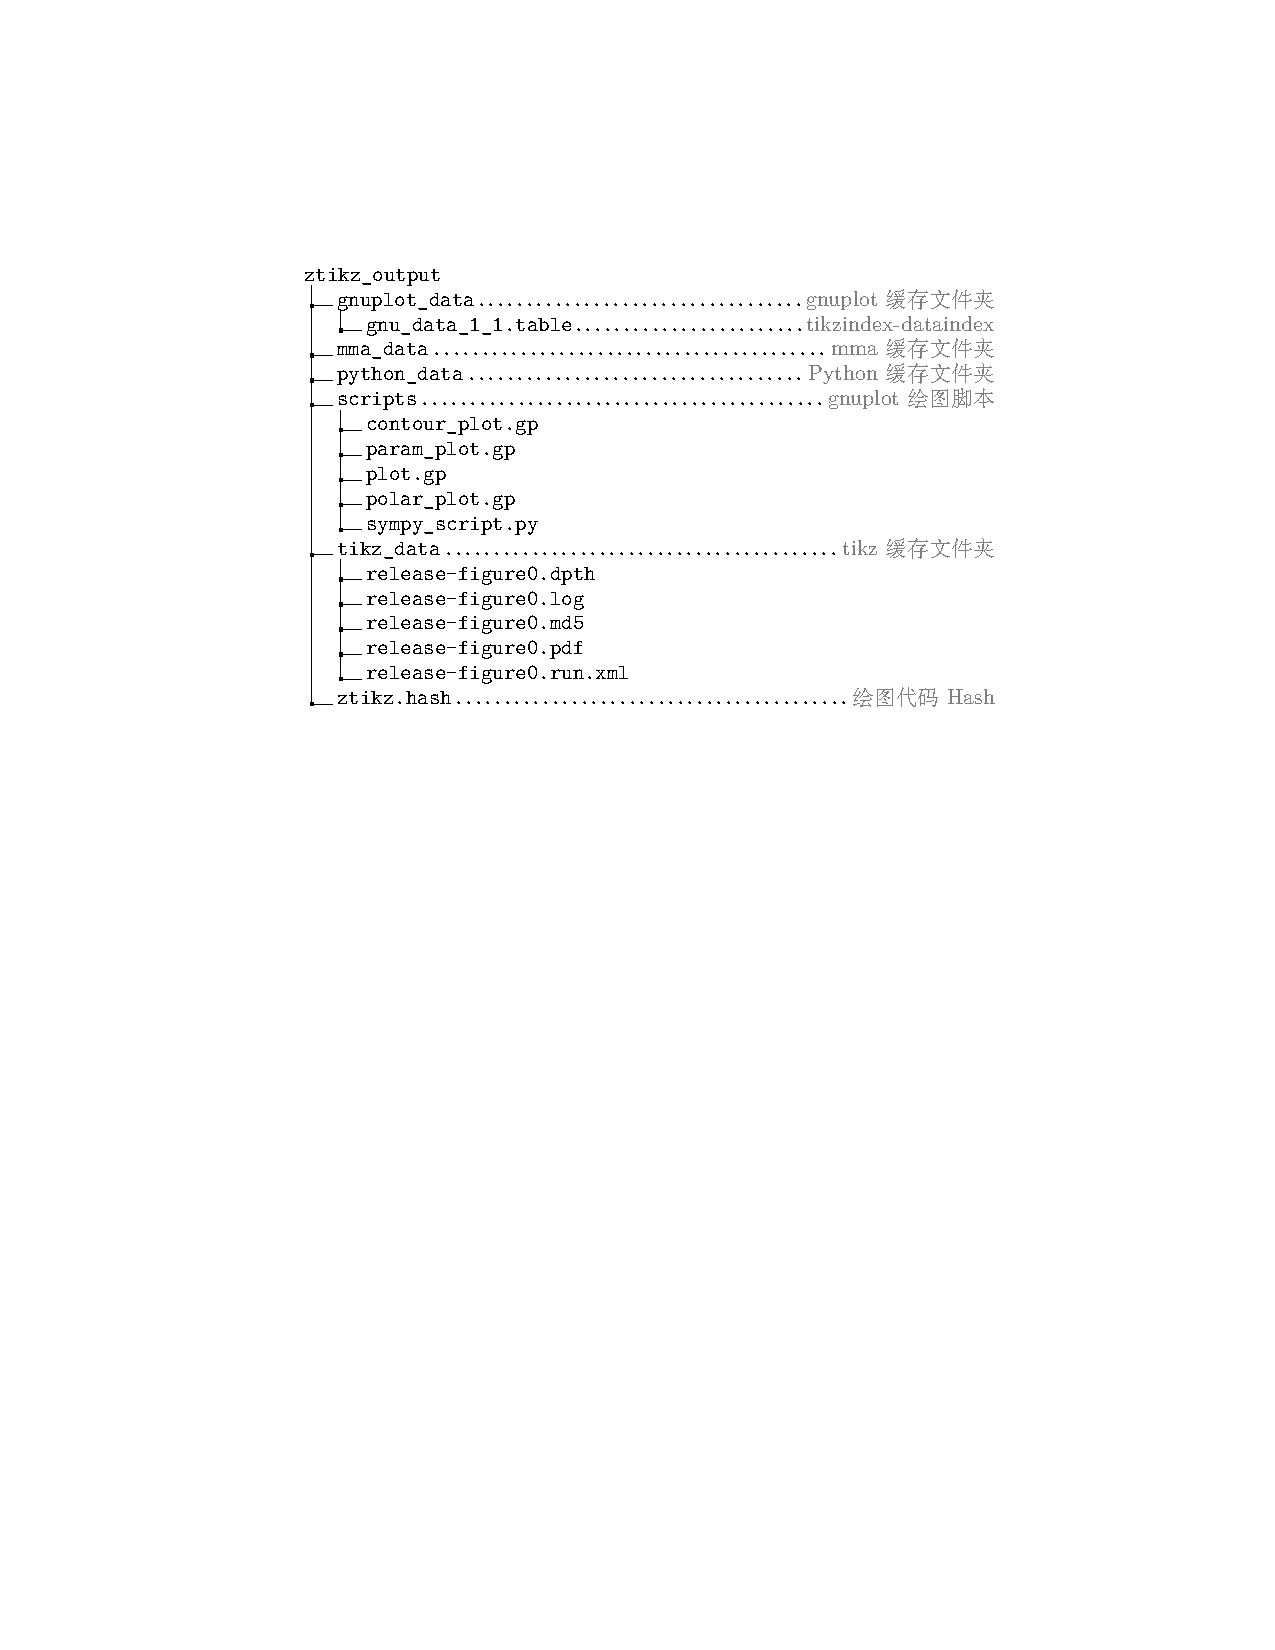
\includegraphics[width=.75\linewidth]{./pics/ztikz_tree.pdf}
    \caption{zTikZ目录结构示意图}
    \label{fig:zTikZ-directory}
\end{figure}

\cmd{tikz_data}中的\cmd{release-figure0.pdf}即为缓存的\cmd{tikzpicture}环境的pdf文件,
对应的\cmd{.md5}文件中:

\begin{codeprint}
\def \tikzexternallastkey {AE7F2539E81C96848ADCCEE3994993D1}%
\end{codeprint}

即保存了\cmd{tikzpicture}环境中代码的Hash Value,当我们改变了\cmd{tikzpicture}环境中的代码时,
这个Hash value就会改变,从而tikz就会再次运行此环境,重新生成图片. 虽说这是tikz自带的功能,但是 
zTikZ中的Cache 机制和这个是十分的类似的,也可以说是一样的. 顺便这里说明命令\cmd{\gnudata}
的用法(在后面区域填充时是即为有用的):

\begin{codeprint}
\gnudata{2} = ./ztikz_output/gnuplot_data/gnu_data_1_2.table
\end{codeprint}

\cmd{\gnudata}参数中的``2''表示此数据是在当前tikzpicture环境中的第二个函数绘图数据; 
每一个已经绘制的函数都会在对应的文件夹下生成一个对应的数据文件,你可以使用此数据文件进行
多种操作:
\begin{itemize}
    \item 绘制此文件:\cmd{\draw plot file{\gnudata{<index>}}}.
    \item 填充此文件对应的曲线:\cmd{\fill[<style>] plot file{\gnudata{<index>}}}.
    \item 绘制此文件对应的散点图:只需在绘制散点图前指定绘制精度即可.
\end{itemize}

\begin{remark}
    目前由于技术原因,\cmd{\ContourPlot}命令生成的数据暂时不可用于后续的填充操作.可以考虑将对应隐函数转化为参数方程形式或极坐标形式. 
    如果你强行使用此类型数据,那么会得到如下的不良输出:
    \begin{figure}[H]
        \centering
        
\includegraphics[width=.3\linewidth]{./pics/contour_data_bug.pdf}
        \caption{ContourPlot Fill Bug}
        \label{fig:ContourPlot Fill Bug}
    \end{figure}
\end{remark}

后续我会解释这个文件夹中其他文件的作用,目前我们先把函数绘制命令\cmd{\Plot}的参数解释清楚。
如果想要设置绘制的函数图形的样式,只需要对其第二个可选项参数进行设置即可,
比如设置为``\textcolor{red}{红色}, \textbf{加粗}''.

\begin{codeprint}
\begin{tikzpicture}
    \Plot[-1.5*pi:pi][red, thick]{sin(x)}
\end{tikzpicture}
\end{codeprint}

\begin{center}
    \begin{tikzpicture}
        \Plot[-1.5*pi:pi][red, thick]{sin(x)}
    \end{tikzpicture}
\end{center}


其实上面的第二个参数的值可以是任何合法的\cmd{\draw[<plot style>]}值, 因为每一个函数
绘制命令均是通过如下的命令实现的:

\begin{codeprint}
% gnuplot data rename, plot and precise reset
\cs_new_protected:Npn \ztikz_gnu_data_plot_cs:nnn #1#2#3 {
    % rename data file
    \int_gadd:Nn \g__gnu_data_index_int {1}
    \tl_set:Nx \l__gnu_data_new_name_tl {
        gnu_data_\int_use:N \g__tikz_env_index_int _
        \int_use:N \g__gnu_data_index_int.table
    }
    \tl_set:Nx \l__gnu_data_full_path_tl {\g__ztikz_gnu_path_tl/\l__gnu_data_new_name_tl}
    \sys_shell_mv:xx {\g__ztikz_gnu_path_tl/gnu_data.table}
                    {\l__gnu_data_full_path_tl}
    % plot data file
    \tl_if_empty:nTF {#3}{
        \draw[#2] plot[smooth] file {\l__gnu_data_full_path_tl};
    }{
        \group_begin:
        \keys_set:nn { ztikz / point } { #3 }
        \draw plot [
            mark = \str_use:N \l__point_type_str, 
            mark~ size = \dim_use:N \l__point_radius_dim,
            mark~ options = {
                rotate  = \fp_use:N \l__point_rotate_angle, 
                opacity = \tl_use:N \l__point_opacity_tl, 
                color   = \tl_use:N \l__point_color_tl,
                ball~ color = \tl_use:N \l__point_color_tl,
            }
        ] file {\l__gnu_data_full_path_tl};
        \group_end:
    }
    % reset precise (default 300 for plot precise)
    \bool_if:cTF {g__#1_precise_bool}{
        \PlotPrecise{#1}{100}
    }{\relax}
}
\end{codeprint}

上述函数\cmd{\ztikz_gnu_data_plot_cs:n} 的第二个参数即为\cmd{\Plot}命令的第二个参数;

\subsection{Show Axis}
最后给我们的图像加上坐标轴等细节: 需要用到绘制坐标轴的\cmd{\ShowAxis}命令, 绘制网格用的\cmd{\ShowGrid}命令,以及
绘制点用的\cmd{\ShowPoint}命令.

其中\cmd{\ShowAxis}\index{\cmd{\ShowAxis}}的参数格式为:\cmd{\ShowAxis[<plot style>]{(start coordinate);(end coordinate)}}.
这里的\cmd{<plot style>}参数采用键值对的形式指定,可用键值对列表以及不同键的默认值可参见如下源码声明:
\begin{codeprint}
% basic tick args
tickStart       .fp_set:N   = \l__start_fp,
tickStart       .initial:n  = { -5 },
tickEnd         .fp_set:N   = \l__end_fp,
tickEnd         .initial:n  = { 5 },
axisRotate      .fp_set:N   = \l__axis_rotate_angle,
axisRotate      .initial:n  = { 0 },
% tick dimension spec
mainStep        .fp_set:N   = \l__main_step_fp,
mainStep        .initial:n  = { 1.0 },
subStep         .fp_set:N   = \l__sub_step_fp,
subStep         .initial:n  = { 0.1 },
mainTickLabel   .tl_set:N   = \l__main_tick_label_tl,
mainTickLabel   .initial:n  = { \fp_use:N {\CurrentFp} },
tickLabelShift  .dim_set:N  = \l__tick_label_shift_dim,
tickLabelShift  .initial:n  = { 0pt },
mainTickLength  .dim_set:N  = \l__main_tick_length_dim,
mainTickLength  .initial:n  = { 4pt },
subTickLength   .dim_set:N  = \l__sub_tick_length_dim,
subTickLength   .initial:n  = { 2pt },
mainTickLabelPosition .tl_set:N  = \l__main_tick_label_position_tl,
mainTickLabelPosition .initial:n = { below },
% color spec
axisColor       .tl_set:N   = \l__axis_color_tl,
axisColor       .initial:n  = { black },
mainTickColor   .tl_set:N   = \l__main_tick_color_tl,
mainTickColor   .initial:n  = { black },
subTickColor    .tl_set:N   = \l__sub_tick_color_tl,
subTickColor    .initial:n  = { black },
mainTickLabelColor .tl_set:N  = \l__main_tick_label_color_tl,
mainTickLabelColor .initial:n = { black },
% tick cross type spec
tickStyle       .choice:,
tickStyle/cross .code:n     = \tl_set:Nn \l__tick_spec_tl { cross },
tickStyle/above .code:n     = \tl_set:Nn \l__tick_spec_tl { above },
tickStyle/below .code:n     = \tl_set:Nn \l__tick_spec_tl { below },
\end{codeprint}

一个自定义\cmd{\ShowAxis}命令示例如下:
\begin{codeprint}
\NewDocumentCommand{\xAxis}{O{-2}O{8}}{
    \ShowAxis[
        tickStart=\fp_eval:n {#1+1}, tickEnd=\fp_eval:n {#2-0.75}, 
        mainStep=1, subStep=.25, 
        axisRotate=0, axisColor=black,
        mainTickColor=black, subTickColor=black,
        mainTickLength=10pt, subTickLength=5pt,
        tickLabelShift=0pt, tickStyle=below, 
        mainTickLabelPosition=below
    ]{(#1, 0); (#2, 0)}
}
\end{codeprint}

从上述zTikZ内置的\cmd{\xAxis}\index{\cmd{\xAxis}}命令可以看出,我们可以指定坐标轴的如下属性:
\begin{itemize}
    \item 主(子)刻度绘制起点/终点
    \item 主(子)刻度颜色设置
    \item 主刻度标签颜色/位置,可选位置有:\cmd{above, below, left, right}
    \item 主(子)刻度长度
    \item 主(子)刻度间隔
    \item 主刻度坐标偏移量
    \item 主(子)刻度旋转角度,请注意调整旋转后标签的位置.
    \item 主(子)刻度样式:\cmd{cross, above, below},分别代表ticks在坐标轴的两侧还是某一侧.
\end{itemize}

\cmd{\ShowAxis}中的第二个参数表示绘制的坐标轴的起点和终点,使用``\cmd{;}''进行分割(zTikZ 中凡是单个参数中含有多个对象的,
分割对象所用到的符号都是``\cmd{;}''). zTikZ内置\cmd{\xAxis,\yAxis}\index{\cmd{\yAxis}}命令,用于绘制两条标准的坐标轴.命令的参数格式为:
\begin{codeprint}
\xAxis[<start>][<end>]
\yAxis[<start>][<end>]
\end{codeprint}

上面的\cmd{<start>, <end>}分别表示$x,y$轴对应的坐标轴绘制的起始,终止点.对应 $x$轴即为:\cmd{(<start>, 0) -- (<end>, 0)}.
$y$轴即交换坐标.

\begin{remark}
    如果在使用\cmd{\ShowAxis}命令时,没有指定可选参数中键\cmd{tickStyle}的值时,那么此时并不会绘制任何的刻度.
\end{remark}

今后读者若需要多次绘制坐标轴及其对应的标签,可以在导言区自定义一个\cmd{\ShowXYAxis}命令,
自动完成坐标轴绘制以及对应的标签。
\begin{codeprint}
\newcommand{\ShowXYAxis}[2]{
    \ShowAxis{(-#1, 0); (#1, 0)}
    \ShowAxis{(0, -#2); (0, #2)}
    \ShowPoint[opacity=0]{(0, 0)}[$O$][below left]
    \ShowPoint[opacity=0]{(#1, 0)}[$x$][below]
    \ShowPoint[opacity=0]{(0, #2)}[$y$][left]
}
\end{codeprint}

然后使用命令\cmd{\ShowXYAxis}即可完成坐标轴的绘制以及对应的标注.第一个参数:$x$的绘制范围为\texttt{[-\#1, \#1]},
第二个参数:$y$的绘制范围为\texttt{[-\#2, \#2]}.默认两轴对称,如果需要更多的样式,请使用\cmd{\ShowAxis}命令进行自定义.

在绘制完坐标轴之后,便可以绘制网格;使用\cmd{\ShowGrid}命令.\cmd{\ShowGrid}\index{\cmd{\ShowGrid}}命令的参数也是和\cmd{\ShowAxis}
命令的参数一样的,只不过此命令中可以指定一个\cmd{step}关键字,用于指定绘制网格的步长(间隔), 如\cmd{step=.5},设置步长为0.5.

\subsection{Show Point}
对应的\cmd{\ShowPoint}\index{\cmd{\ShowPoint}}命令的参数格式为:

\begin{codeprint}
\ShowPoint[<marker option>]{(coordinate 1); (coordinate 2); ...}[<label 1>; <label2>; ...][<position>]
\end{codeprint}

上述的\cmd{<marker option>>}\index{\cmd{<marker option>}}通过\cmd{<key>-<value>}的格式进行指定, 可用的\cmd{<key>-<value>}列表为:

\begin{itemize}
    \item \cmd{type}: zTikZ库已经加载\cmd{pgfmarkers}库,所以任何在此库中的形状均为有效值, 
        默认为实心circle.\cmd{type=*}. 可以参见\cref{fig:point-marker},截取自pgf手册.
    \item \cmd{radius}: \cmd{<dimension>}, 点的半径,默认为 1pt.
    \item \cmd{color}: \cmd{<color>}, 点的颜色, 默认为black.
    \item \cmd{opacity}: \cmd{<float value>}, 点的透明度,默认为1,即不透明.
    \item \cmd{rotate}: marker的旋转角度, 默认为0.
\end{itemize}

\begin{figure}
    \centering
    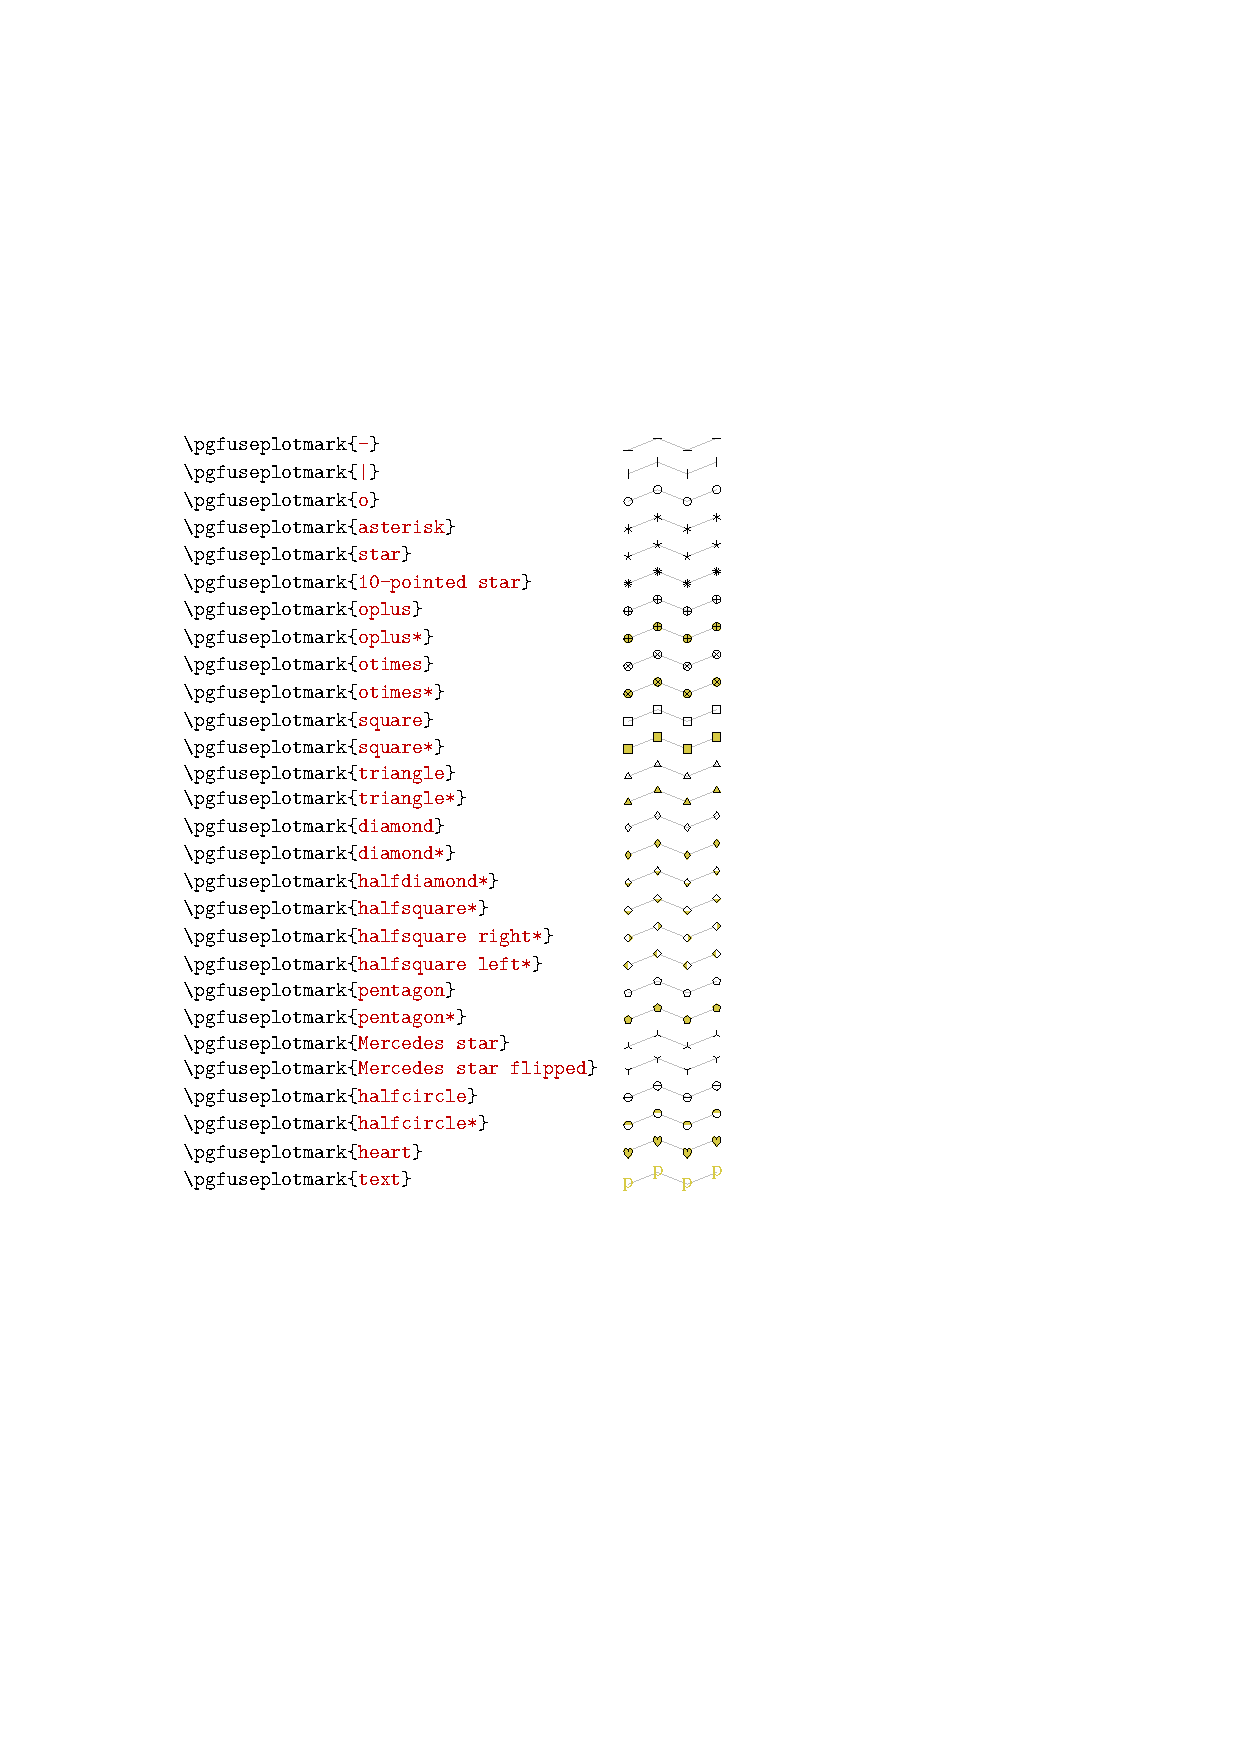
\includegraphics[width=.85\linewidth]{./pics/point_marker.pdf}
    \caption{Point Marker}
    \label{fig:point-marker}
\end{figure}

终于,现在我们可以给出一个相对完整的代码(包括\cmd{<marker option>}对应的用法):

\begin{codeprint}
\begin{tikzpicture}[>=Latex]
    \xAxis[-5][5]
    \yAxis[-2][5]
    \Plot[-1.5*pi:pi][red, thick]{sin(x)}
    \ShowGrid[gray, step=1, opacity=.5]{(-5, -2); (5, 5)}
    % marker option
    \PlotPrecise{plot}{10}
    \Plot[-1.5*pi:pi][red, thick][type=ball, color=red]{sin(x)+.75}
    % show point
    \ShowPoint[color=teal, radius=2pt, type=pentagon*, opacity=.8, rotate=60]
        {(0, 0); (3.1415926, 0)}[$O=(0, 0)$; $(\pi, 0)$][above right=4em and 0em, font=\small]
\end{tikzpicture}
\end{codeprint}

\begin{center}
\begin{tikzpicture}[>=Latex]
    \xAxis[-5][5]
    \yAxis[-2][5]
    \Plot[-1.5*pi:pi][red, thick]{sin(x)}
    \ShowGrid[gray, step=1, opacity=.5]{(-5, -2); (5, 5)}
    % marker option
    \PlotPrecise{plot}{10}
    \Plot[-1.5*pi:pi][red, thick][type=ball, color=red]{sin(x)+.75}
    % show point
    \ShowPoint[color=teal, radius=2pt, type=pentagon*, opacity=.8, rotate=60]
        {(0, 0); (3.1415926, 0)}[$O=(0, 0)$; $(\pi, 0)$][above right=4em and 0em, font=\small]
\end{tikzpicture}
\end{center}

\begin{leftbar}
\noindent \textbf{注意:}zTikZ中的命令都不需要你使用``\cmd{;}''去结束绘制.
\end{leftbar}

更多的关于Marker的选项和用法,请参见如下示例:
\begin{codeprint}
\begin{tikzpicture}[>=Latex]
    \xAxis[-5][5]
    \yAxis[-5][5]
    \ShowGrid[gray, step=1, opacity=.5]{(-5, -2); (5, 5)}
    \PlotPrecise{plot}{10}
    \Plot[-1.5*pi:pi][red, thick][type=ball, color=red]{sin(x)}

    \PlotPrecise{polar}{20}
    \PolarPlot[0:10*pi][orange][type=ball, color=red]{0.1*t}

    \PlotPrecise{contour}{40}
    \ContourPlot[-4:4][green][type=ball, color=red]{x**2/9+y**2/4-1}

    \PlotPrecise{param}{40}
    \ParamPlot[0:2*pi][red, name path=ellipse][type=ball, color=red]{2*sin(t), 3*cos(t)}
\end{tikzpicture}
\end{codeprint}

\subsection{Contour Plot}
其余的几个函数绘制命令,稍微值得一提的是命令\cmd{\ContourPlot}\index{\cmd{\ContourPlot}}, 其参数格式为:

\begin{codeprint}
\ContourPlot[<plot domain>][<plot style>][<marker options>]{<function>}
\end{codeprint}

但是因为是 contour plot, 所以它的定义域的指定格式是比较特别的; 比如绘制的定义为:
$-3<x<\pi$ 并且 $-1.5<y<e$. 那么在指定其\cmd{<plot domain>}时应该写为
\cmd{-3:pi;-1.5:exp(1)}.

\begin{leftbar}
\noindent 由于zTikZ的这部分功能都是以gnuplot为基础,所以只要是gnuplot支持的函数,gnuplot内置的任何常数;
你都可以在zTikZ中使用;这里给不熟悉gnuplot的你们推荐一份7页的gnuplot快速
入门清单:\href{http://www.gnuplot.info/docs_4.0/gpcard.pdf}{gnuplot card}
\end{leftbar}

这里就给出一个\cmd{\ContourPlot}的例子,对应的绘图代码见后面:

\begin{center}
    \begin{tikzpicture}[>=Latex, scale=.5]
        \ShowAxis{(-5, 0); (5, 0)}
        \ShowAxis{(0, -5); (0, 5)}
        \ContourPlot[-3:pi; -3:exp(1)][red]{x**2/16 + y**2/10 - 1}
    \end{tikzpicture}
\end{center}

\begin{codeprint}
\begin{tikzpicture}[>=Latex, scale=.5]
    \ShowAxis{(-5, 0); (5, 0)}
    \ShowAxis{(0, -5); (0, 5)}
    \ContourPlot[-3:pi; -3:exp(1)][red]{x**2/16 + y**2/10 - 1}
\end{tikzpicture}
\end{codeprint}

对于\cmd{\ContourPlot}还有一点提醒:如果要绘制 $x^2/4+y^2/9=1$,那么你只需要输入\cmd{x**2/4+y**2/9-1}即可;
所以由此也暗示了此命令的另一个用法,用于绘制水平线($y=c$)和竖直线($x=c$). 仍然可以使用前面的\cmd{<plot domain>}
控制 $x,y$的范围,比如绘制 $x=1, -1<y<1$. 那么对应的命令就是(第一个参数范围只要包含 $x=1$即可):

\begin{codeprint}
\ContourPlot[0:2; -1:1][red, dashed]{x-1}
\end{codeprint}

\subsection{Intersection and Plot Precise}
我们还有两个命令没有讲到:\cmd{\ShowIntersection}\index{\cmd{\ShowIntersection}}, \cmd{\PlotPrecise}\index{\cmd{\PlotPrecise}};
其中\cmd{\ShowIntersection}
命令的参数格式为:

\begin{codeprint}
\ShowIntersection{<path 1>; <path 2>}[<number of points>]
\end{codeprint}

指定tikz中path名称并显示交点方法示例, 我们分别指定两条叫做\cmd{line1, line2}的路径,并显示它们二者的交点.

\begin{codeprint}
\begin{tikzpicture}[>=Latex]
    \ShowAxis{(-2, 0); (4, 0)}
    \ShowAxis{(0, -2); (0, 4)}
    \Plot[1:3][name path=line1]{2*x-3}
    \Plot[0:3][name path=line2]{-x+3}
    \ShowIntersection[color=red]{line1; line2}{1}

    % 可以使用如下的语句
    % \path[name intersections={of=line1 and line2}];
    % \ShowPoint[color=red] {(intersection-1)}
\end{tikzpicture}
\end{codeprint}


\begin{center}
    \begin{tikzpicture}[>=latex]
        \ShowAxis{(-2, 0); (4, 0)}
        \ShowAxis{(0, -2); (0, 4)}
        \Plot[1:3][name path=line1]{2*x-3}
        \Plot[0:3][name path=line2]{-x+3}
        \ShowIntersection[color=red]{line1; line2}{1}
    \end{tikzpicture}
\end{center}


\cmd{\PlotPrecise}\index{\cmd{\PlotPrecise}}命令的参数格式为:
\begin{codeprint}
\PlotPrecise{<plot type>}[<change domain>]{<samples-int>}
\end{codeprint}

支持的\cmd{<plot type>}有 \cmd{plot, param, contour, polar}, 分别设置对应的
命令\cmd{\Plot, \ParamPlot, \ContourPlot, \PolarPlot}的采样精度. 采样精度的设置
分为两种,临时和永久,临时改变(只改变下一个命令的采样精度)的方法是在命令的第二个参数中
填入\cmd{[once]}, 而如果填入不是\cmd{once},那么接下来的所有同种\cmd{<plot type>}的命令
的采样精度都会改变. 下面给出一个采样精度设置的例子, 绘制在区间$[-2, 2]$上的
函数 $y=3\sin(1/x)$在采样精度分别为50和1000的图像:

\parbox{.48\linewidth}{
    \centering
    \begin{tikzpicture}
        \PlotPrecise{plot}{50}
        \Plot[-2:2]{3*sin(1/x)}
    \end{tikzpicture}
}
\parbox{.48\linewidth}{
    \centering
    \begin{tikzpicture}
        \PlotPrecise{plot}{1000}
        \Plot[-2:2]{3*sin(1/x)}
    \end{tikzpicture}
}


\section{Statistic Plot}
\subsection{Stairs Plot}
了解完用户曲线绘制的一系列Plot命令后,现在开始介绍和统计相关的几个绘图命令:
\cmd{\ListPlot}\index{\cmd{\ListPlot}}, \cmd{\StairsPlot}\index{\cmd{\StairsPlot}}, 
\cmd{\StemPlot}\index{\cmd{\StemPlot}}, \cmd{\BarPlot}\index{\cmd{\BarPlot}}, \cmd{\ShadePlot}\index{\cmd{\ShadePlot}}.
这几个命令在本节开篇已经介绍了其大致的功能. 本节主要聚焦于怎么使用这几个命令. 由于除\cmd{\ShadePlot,\ListPlot}外,其余3者的用法完全一致,
不同的仅仅为第一个可选参数的意义. 其中\cmd{\ListPlot}仅仅只需把对应的绘制命令中\cmd{opacity=0}即可,本节便以\cmd{\StairsPlot}为例,
讲解这三者的用法。同时也会给出3者的具体示例.

\cmd{\StairsPlot}主要用于绘制阶梯图,命令格式为:
\begin{codeprint}
\StairsPlot[<stairs option>][<draw option>][<marker option>]{<data>}
\end{codeprint}

第一个可选参数的可选值有:\cmd{plot-left(plot-right);jump-right(plot-left)},我们以``;''进行两个配置项的分割.
第一个配置项\cmd{plot-<.>}表示在绘制数据点时水平线取值为左值还是右值.第二个配置项\cmd{jump-<.>}表示在绘制数据点时
跳过左侧还是右侧的垂直线,为空时默认绘制两侧的垂直线. 

\begin{remark}
    如果两个配置项\cmd{plot-<.>, jump-<.>}均为空,那么此时绘制的图像为通过线段相连的散点图
\end{remark}

其中必选参数\cmd{<data>}表示要可视化的数据文件,可以手动输入数据文件地址,也可以使用前文定义的\cmd{\gnudata{<index>}}命令
用于引用前面已经生成的数据,\textbf{这也就意味着要使用此命令,必须先产生对应的数据}.一个绘制样例如\cref{fig:stairs-plot}:

\begin{codeprint}
\begin{tikzpicture}
    \ShowGrid[step=1]{(-5, -5); (5, 5)}
    %% \StairsPlot
    % 1. connected using piecewise constant series of lines
    \begin{scope}[yshift=1cm]
        \StairsPlot[plot-left;][red]{./data/sine.data}
        \node[left] at (-3.14, 0) {plot left(default)};
    \end{scope}
    \begin{scope}[yshift=-1cm]
        \StairsPlot[plot-right;][orange]{./data/sine.data}
        \node[left] at (-3.14, 0) {plot right};
    \end{scope}
    % 2. plot segment (non-connected series of lines)      
    \begin{scope}[yshift=2cm]
        \StairsPlot[;jump-left][teal][type=ball, color=teal]{./data/sine.data}
        \node[left] at (-3.14, 0) {jump left};
    \end{scope}
    \begin{scope}[yshift=-2cm]
        \StairsPlot[;jump-right][cyan][type=ball, color=cyan]{./data/sine.data}
        \node[left] at (-3.14, 0) {jump right};
    \end{scope}
\end{tikzpicture}
\end{codeprint}

\begin{figure}
    \centering
    \begin{tikzpicture}
        \ShowGrid[step=1]{(-5, -5); (5, 5)}
        %% \StairsPlot
        % 1. connected using piecewise constant series of lines
        \begin{scope}[yshift=1cm]
            \StairsPlot[plot-left;][red]{./data/sine.data}
            \node[left] at (-3.14, 0) {plot left(default)};
        \end{scope}
        \begin{scope}[yshift=-1cm]
            \StairsPlot[plot-right;][orange]{./data/sine.data}
            \node[left] at (-3.14, 0) {plot right};
        \end{scope}
        % 2. plot segment (non-connected series of lines)      
        \begin{scope}[yshift=2cm]
            \StairsPlot[;jump-left][teal][type=ball, color=teal]{./data/sine.data}
            \node[left] at (-3.14, 0) {jump left};
        \end{scope}
        \begin{scope}[yshift=-2cm]
            \StairsPlot[;jump-right][cyan][type=ball, color=cyan]{./data/sine.data}
            \node[left] at (-3.14, 0) {jump right};
        \end{scope}
    \end{tikzpicture}
    \caption{stairs-plot}
    \label{fig:stairs-plot}
\end{figure}

其余的两个相似命令\cmd{\StemPlot, \BarPlot}的参数格式为:
\begin{codeprint}
\StairsPlot[<stem/bar option>][<draw option>][<marker option>]{<data>}
\end{codeprint}

这里主要说明第一个可选参数的可选值列表,默认值以及其对应的实际含义:

\begin{multicols}{2}
\begin{itemize}
    \item \cmd{\StemPlot}
        \begin{itemize}
            \item \cmd{x}:表示绘制一个垂直于$x$轴上的火柴棍图
            \item \cmd{x}:表示绘制一个垂直于$y$轴上的火柴棍图
            \item \cmd{o}:表示绘制一个中心为原点 $O=(0,0)$的火柴棍图
            \item 若为空值,那么默认和\cmd{x}参数时的情形一致
        \end{itemize}
    \item \cmd{\BarPlot}
        \begin{itemize}
            \item \cmd{x}:表示绘制一个垂直于$x$轴上的{\bf 离散}柱形图
            \item \cmd{y}:表示绘制一个垂直于$y$轴上的{\bf 离散}柱形图
            \item \cmd{xc}:表示绘制一个垂直于$x$轴上的{\bf 连续}柱形图
            \item \cmd{yc}:表示绘制一个垂直于$y$轴上的{\bf 连续}柱形图
            \item 若为空值,那么默认和\cmd{x}参数时的情形一致
        \end{itemize}
\end{itemize}
\end{multicols}

\subsection{Stem/Bar Plot}
下面各处这两个命令的一个简单示例,见\cref{fig:bar-plot}, \cref{fig:stem-plot}:
\begin{codeprint}
\begin{tikzpicture}
    \ShowGrid[step=1]{(-5, -5); (5, 5)}
    %% \StemPlot
    % 1. xcomb
    \begin{scope}[yshift=-3cm]
        \StemPlot[x][red][type=*, color=red]{./data/sine.data}
        \node[left] at (-3.14, 0) {xcomb};
    \end{scope}
    % 2. ycomb
    \begin{scope}[yshift=0cm]
        \StemPlot[y][orange][type=*, color=orange]{./data/sine.data}
        \node[left] at (-3.14, 0) {ycomb};
    \end{scope}
    % 3. polar comb
    \begin{scope}[yshift=3cm]
        \StemPlot[o][cyan][type=*, color=cyan]{./data/sine.data}
        \node[left] at (-2, 0) {polar comb};
    \end{scope}
\end{tikzpicture}
\end{codeprint}

\begin{figure}[!htb]
    \centering
    \begin{tikzpicture}
        \ShowGrid[step=1]{(-5, -5); (5, 5)}
        %% \StemPlot
        % 1. xcomb
        \begin{scope}[yshift=-3cm]
            \StemPlot[x][red][type=*, color=red]{./data/sine.data}
            \node[left] at (-3.14, 0) {xcomb};
        \end{scope}
        % 2. ycomb
        \begin{scope}[yshift=0cm]
            \StemPlot[y][orange][type=*, color=orange]{./data/sine.data}
            \node[left] at (-3.14, 0) {ycomb};
        \end{scope}
        % 3. polar comb
        \begin{scope}[yshift=3cm]
            \StemPlot[o][cyan][type=*, color=cyan]{./data/sine.data}
            \node[left] at (-2, 0) {polar comb};
        \end{scope}
    \end{tikzpicture}
    \caption{stem-plot}
    \label{fig:stem-plot}
\end{figure}

\begin{codeprint}
\begin{tikzpicture}
    \ShowGrid[step=1, color=gray, opacity=.5]{(-5, -5); (5, 5)}
    % 1. xbar
    \begin{scope}[yshift=-1cm]
        \BarPlot[x][red, pattern=north west lines, pattern color=red]{./data/sine.data}
        \node[left] at (-3.14, 0) {xbar};
    \end{scope}
    % 2. ybar
    \begin{scope}[yshift=1cm]
        \BarPlot[y][orange, pattern=north west lines, pattern color=orange]{./data/sine.data}
        \node[left] at (-3.14, 0) {ybar};
    \end{scope}
    % 3. xbar interval (fill) 
    \begin{scope}[yshift=4cm]
        \BarPlot[xc][cyan, pattern=north west lines, pattern color=cyan]{./data/sine.data}
        \node[left] at (-3.14, 0) {xbar continuous};
    \end{scope}
    % 3. ybar interval (fill) 
    \begin{scope}[yshift=-3cm]
        \BarPlot[yc][green, pattern=north west lines, pattern color=green]{./data/sine.data}
        \node[left] at (-3.14, 0) {ybar continuous};
    \end{scope}
    % annotate
    \node at (2.25 ,-4.5) {Optional args:bar width, bar shift};
\end{tikzpicture}    
\end{codeprint}

\begin{figure}[!htb]
    \centering
    \begin{tikzpicture}
        \ShowGrid[step=1, color=gray, opacity=.5]{(-5, -5); (5, 5)}
        % 1. xbar
        \begin{scope}[yshift=-1cm]
            \BarPlot[x][red, pattern=north west lines, pattern color=red]{./data/sine.data}
            \node[left] at (-3.14, 0) {xbar};
        \end{scope}
        % 2. ybar
        \begin{scope}[yshift=1cm]
            \BarPlot[y][orange, pattern=north west lines, pattern color=orange]{./data/sine.data}
            \node[left] at (-3.14, 0) {ybar};
        \end{scope}
        % 3. xbar interval (fill) 
        \begin{scope}[yshift=4cm]
            \BarPlot[xc][cyan, pattern=north west lines, pattern color=cyan]{./data/sine.data}
            \node[left] at (-3.14, 0) {xbar continuous};
        \end{scope}
        % 3. ybar interval (fill) 
        \begin{scope}[yshift=-3cm]
            \BarPlot[yc][green, pattern=north west lines, pattern color=green]{./data/sine.data}
            \node[left] at (-3.14, 0) {ybar continuous};
        \end{scope}
        % annotate
        \node at (0, -4.5) {Optional args for the Second:bar width, bar shift};
    \end{tikzpicture}
    \caption{bar-plot}
    \label{fig:bar-plot}
\end{figure}

\subsection{List Plot}
然后讲解一下怎么绘制散点图,以\cmd{\Plot, \PolarPlot}命令为例,见\cref{fig:list-plot}:
\begin{codeprint}
\begin{tikzpicture}
    \ShowGrid[step=1, color=gray, opacity=.5]{(-5, -5); (5, 5)}
    \begin{scope}[yshift=-2cm]
        \PlotPrecise{plot}{10}
        \Plot[-pi:pi][opacity=0, red][type=o, color=red]{sin(x)}
    \end{scope}
    \begin{scope}[yshift=3cm]
        \PlotPrecise{polar}{15}
        \PolarPlot[0:2*pi][opacity=0, orange][type=square, color=orange]{1-sin(t)}
    \end{scope}
    % continuous condition
    \Plot[-pi:pi][red]{sin(x)}
    \PolarPlot[0:2*pi][orange]{1-sin(t)}
\end{tikzpicture}
\end{codeprint}

\begin{figure}[!htb]
    \centering
    \begin{tikzpicture}
        \ShowGrid[step=1, color=gray, opacity=.5]{(-5, -5); (5, 5)}
        \begin{scope}[yshift=-2cm]
            \PlotPrecise{plot}{10}
            \Plot[-pi:pi][opacity=0, red][type=o, color=red]{sin(x)}
        \end{scope}
        \begin{scope}[yshift=3cm]
            \PlotPrecise{polar}{15}
            \PolarPlot[0:2*pi][opacity=0, orange][type=square, color=orange]{1-sin(t)}
        \end{scope}
        % continuous condition
        \Plot[-pi:pi][red]{sin(x)}
        \PolarPlot[0:2*pi][orange]{1-sin(t)}
    \end{tikzpicture}
    \caption{list-plot}
    \label{fig:list-plot}
\end{figure}

\subsection{Shade Plot}
最后讲解\cmd{\ShadePlot}命令,参数格式为:
\begin{codeprint}
\ShadePlot[<shade mode>][<box distance>]{<data>}
\end{codeprint}

其中第一个参数\cmd{<shade mode>}使用命令\cmd{\ztikzShadeMode}命令进行声明,此命令的一个样例为(zTikZ默认shade模式):
\begin{codeprint}
\ztikzShadeMode{defaultMode}{horizontal}{white,black}
\end{codeprint}

\cmd{\ztikzShadeMode}的第二个参数可以为\cmd{vertical},表示垂直渐变.第三个参数中的颜色也可以超过两个。一个具体的
使用样例,见\cref{fig:shade-plot}:

\begin{codeprint}
% compile with "\usepackage[external=false]{ztikz}"
\ztikzShadeMode{newyMode}{vertical}{white,black}
\begin{tikzpicture}
    \ShowGrid[step=1, color=gray, opacity=.5]{(-5, -5); (5, 5)}
    \ShadePlot[newyMode][10pt]{./data/sine.data}
\end{tikzpicture} 
\end{codeprint}

\begin{figure}[!htb]
    \centering
    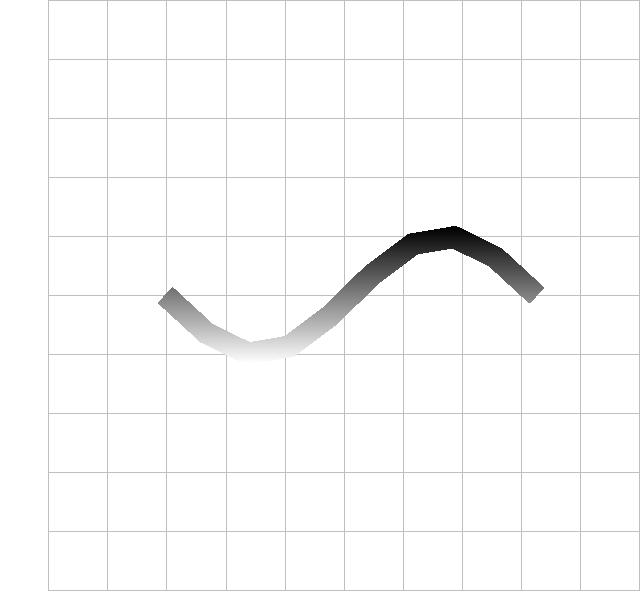
\includegraphics[width=.75\linewidth]{./pics/ztikz_example_5.pdf}
    \caption{shade-plot}
    \label{fig:shade-plot}
\end{figure}

\begin{remark}
目前此命令可能会存在部分的潜在问题,请谨慎使用此命令(比如此命令不支持\cmd{external}库的缓存功能). 
如果想要创建一个shade区域,直接使用 \cmd{\shade}命令来代替\cmd{\fill}命令即可.在指定\cmd{\shade[<shade mode>] ...}命令
中的\cmd{<shade mode>}时可以为:\cmd{top color=red, bottom color=blue}或者是\cmd{left color=red, right color=blue}.
\end{remark}


\section{Polygon}
目前zTikZ的\cmd{Polygon}命令已经开发完毕, 此命令主要用于绘制正多边形。命令格式如下:
\begin{codeprint}
\Polygon[<options>]{<edges>}
\end{codeprint}

第二个参数是比较简单的,只需要输入一个正整数即可,表示多边形的边数. 第一个参数是一个可选参数,可以指定旋转角度,多边形的边长,边的颜色
多边形填充样式与颜色,顶点样式等.可用的键值对以及默认值如下:

\begin{codeprint}
\keys_define:nn { ztikz / polygon }{
    radius       .fp_set:N  = \l__polygon_radius_fp,
    radius       .initial:n = { 1 },
    edgeColor    .tl_set:N  = \l__polygon_edge_color_tl,
    edgeColor    .initial:n = { black },
    fillColor    .tl_set:N  = \l__polygon_fill_color_tl,
    fillColor    .initial:n = { white },
    fillOpacity  .fp_set:N  = \l__polygon_fill_opacity_fp,
    fillOpacity  .initial:n = { 0 },
    rotate       .fp_set:N  = \l__polygon_rotate_angle,
    rotate       .initial:n = { 0 },
    shift        .tl_set:N  = \l__polygon_shift_tl,
    shift        .initial:n = { (0,0) },
    marker       .tl_set:N  = \l__polygon_marker_option_tl,
    marker       .initial:n = { },
}
\end{codeprint}

这里指的说一下的参数是:\cmd{marker},此参数中可以填入任意合法的\cmd{<marker option>}键值对,一下为一个简单示例:
\begin{codeprint}
\Polygon [
    radius=2, 
    shift={(3,0)}, 
    rotate=60, 
    marker={type=ball, color=red}, 
    edgeColor=teal, 
    fillColor=red, 
    fillOpacity=0.5
]{3}
\end{codeprint}

\begin{remark}
    多边形的变数必须为整数,同时再说明一下键\cmd{shift}的含义:合法的值为一个使用``()''包括的向量,表示 
    整个多边形的平移量.比如\cmd{shift={(3,-4)}}表示整个多边形向右平移3个单位,象下平移4个单位. 不要忘记向量
    外层的\texttt{\{\}}.
\end{remark}

在讲述了\cmd{\Polygon}命令的用法后,下面给出一个简单的使用样例,见\cref{fig:polygon}:
\begin{codeprint}
\begin{tikzpicture}
    \ShowGrid[step=1, color=gray, opacity=.5]{(-5, -5); (5, 5)}
    \Polygon[shift={(0, 0)}]{3}
    \Polygon[shift={(3, 0)}, fillColor=red, fillOpacity=.5]{4}
    \Polygon[shift={(0, 3)}, edgeColor=green, fillOpacity=.3, marker={type=ball, color=green}, rotate=18]{5}
    \Polygon[shift={(-3,0)}, fillColor=orange, fillOpacity=.75]{6}
    \Polygon[shift={(0,-3)}, fillColor=teal, fillOpacity=.5, marker={type=oplus*, color=teal}]{8}
\end{tikzpicture}
\end{codeprint}

\begin{figure}[!htb]
    \centering
    \begin{tikzpicture}
        \ShowGrid[step=1, color=gray, opacity=.5]{(-5, -5); (5, 5)}
        \Polygon[shift={(0, 0)}]{3}
        \Polygon[shift={(3, 0)}, fillColor=red, fillOpacity=.5]{4}
        \Polygon[shift={(0, 3)}, edgeColor=green, fillOpacity=1, marker={type=ball, color=green}, rotate=18]{5}
        \Polygon[shift={(-3,0)}, fillColor=orange, fillOpacity=.75]{6}
        \Polygon[shift={(0,-3)}, fillColor=teal, fillOpacity=.5, marker={type=diamond*, color=red}]{8}
    \end{tikzpicture}
    \caption{polygon}
    \label{fig:polygon}
\end{figure}


\begin{remark}
    在填充多边形时,必须同时指定键\cmd{fillOpacity}的值,因为此值默认为0;
    如果你想要填充一个透明度为50\%的多边形,那么你可以使用\cmd{fillOpacity=0.5}来实现.
\end{remark}



\section{python/matplotlib}
python绘图是比较就简单的,zTikZ提供了用于python绘图的\cmd{pyfig}\index{\cmd{pyfig}}环境。
此环境需要填入两个参数,参数格式为:

\begin{codeprint}
\begin{pyfig}[<width>]{<export file name>}
% your code
\end{pyfig}
\end{codeprint}

其中的\cmd{<width>}参数是命令\cmd{\includegraphics[<width>]{}}中的参数,比如你可以输入\cmd{width=.75\linewidth}. 
再指定必要的参数后,你可以直接在环境中输入Python代码. 下面即为一个示例:

\begin{codeprint}
\begin{pyfig}[width=.45\linewidth]{pycode.py}
import matplotlib 
matplotlib.use('Agg')
from matplotlib import pyplot as plt
plt.rcParams['font.sans-serif'] = ['FangSong']  
plt.rcParams['axes.unicode_minus'] = False
import numpy as np

x = np.linspace(0, 2*np.pi, num = 80)
y = np.sin(x)*np.cos(x)+.2
plt.plot(x, y)
\end{pyfig}
\end{codeprint}

你不需要在其中输入图片的保存指令\cmd{plt.savefig("")}, zTikZ会自动在此环境后面加上对应的
图片保存指令。这个环境的返回结果为:\cmd{\includegraphics[width=.45\linewidth]{pycode.py.pdf}},
所以你可以把这个环境嵌套在任何的浮动环境,比如\cmd{figure, table}中. 

在命令行中第一次编译时你会看到如下的日志:
\begin{codeprint}
current hash is FF7B5ECDBF52AA95DF921FCC076F9021
current hash is unique --> recorded
\end{codeprint}

上述日志说明,zTikZ已经识别到这是一个新的python环境,并且保存了这个环境中绘图代码的Hash值;
然后,第二次编译此文档时,你会在输出的日志中定位到如下的输出:
\begin{codeprint}
current hash is FF7B5ECDBF52AA95DF921FCC076F9021
skip recompile by python, using the cache picture 1
\end{codeprint}

这就说明,由于你的python绘图部分的源代码没有改变,然后zTikZ就直接采用了上一次编译的缓存图片,跳过了重新编译这一步;
上面环境的运行结果为:

\begin{figure}[!htb]
    \centering
\begin{pyfig}[width=.75\linewidth]{pycode.py}
import matplotlib 
matplotlib.use('Agg')
from matplotlib import pyplot as plt
plt.rcParams['font.sans-serif'] = ['FangSong']  
plt.rcParams['axes.unicode_minus'] = False
import numpy as np

x = np.linspace(0, 2*np.pi, num = 80)
y = np.sin(x)*np.cos(x)+.2
plt.plot(x, y)
\end{pyfig}
    \caption{Python绘图示例 1}
    \label{fig:py-fig-1}
\end{figure}

这里再给一个Python绘图环境的示例,绘制了一个简单的来自Matplotlib官方的三维图像. 
其实这里给出这个例子,就是为了让读者明白,尽管目前zTikZ还没有支持便捷的三维矢量图形绘制,
但是你可以使用Python生成对应的3维矢量图;虽然,你可能需要再去学习Python中Matplotlib的
相关语法,但是这是简单的.

\begin{figure}[!htb]
    \centering
    \input{./data/pyfig_II.mpl}
    \caption{Python绘图示例 2}
    \label{fig:py-fig-2}
\end{figure}

\begin{remark}
由于python是依靠缩进来识别代码结构的,所以在书写这部分的代码时,不能够人工添加缩进,在书写的时候
需写为下面这样:
\begin{center}
    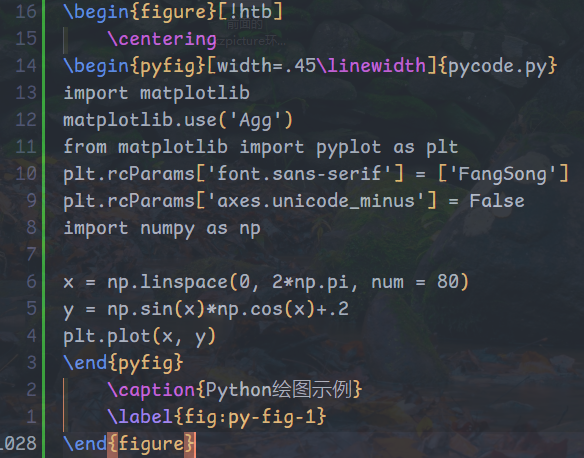
\includegraphics[width=.45\linewidth]{./pics/pyfig_example.png}
\end{center}

如果你实在是需要缩进,那么在这里我推荐另外一种可以使用缩进的方法:把\cmd{pyfig}环境连同其内部代码保存在另外一个文件中,
比如这里我保存为\cmd{pycode.mpl},然后在\cmd{figure}环境中使用\cmd{\input{pycode.mpl}}引入此部分的代码。如下:
\begin{codeprint}
\begin{figure}
    \centering
    \input{./data/pycode.mpl}
    \caption{Python Figure}
    \label{fig:pyfig-1}
\end{figure}
\end{codeprint}
\end{remark}


\section{mathematica}
其实使用mathematica进行绘图这个部分和前面的使用Python绘图是差不多的,zTikZ提供了一个
\cmd{wolframGraphics}\index{\cmd{wolframGraphics}}环境用于使用mathematica绘图. 与之前的\cmd{pyfig}环境不同的是,此时你需要手动加入
图片的保存路径;路径的前缀为:\cmd{./ztikz_output/mma_data/<figure name>}. 为何这里这个部分
我不使用zTikZ自动完成? 由于mathematica绘图代码中可能存在着多幅图形的情况,需要使用\cmd{Show}命令
组合成为一个图,那么这个组合方式就是千变万化的了。所以为了给用户提供给更多的自由操作的空间。
这里的图片保存命令由用户自己书写. 并且上述的\cmd{<figure name>}只能写为\cmd{<wls script name>.pdf}
的形式;比如你的WolframScript脚本名称为\cmd{mma_1.wls},那么你的\cmd{<figure name>}只能写为
\cmd{mma_1.wls.pdf},其中的图片格式可以自己指定,比如为\cmd{.png, .jpg, .mbp}等. 此环境同样是加入了Cache机制的,
下面给出一个具体的使用案例:

\begin{codeprint}
\begin{wolframGraphics}[width=.4\linewidth]{mma_1.wls}
    plotFunction[fun_, xlimits_, ylimits_] := ContourPlot[fun, 
        xlimits, ylimits,
        ContourStyle->{
            RGBColor["#00C0A3"], 
            Thickness[0.004]
        },
        AspectRatio->((xlimits[[2]]//Abs) + (xlimits[[3]]//Abs))/((ylimits[[2]]//Abs) + (ylimits[[3]]//Abs)), 
        AxesOrigin->{0,0}, 
        Axes->True,
        Frame->False,
        AxesStyle->Arrowheads[{0, 0.03}],
        AxesLabel->{"x", "y"},
        PlotRange -> Full
    ]
    
    xlimits = {x, -3, 6};
    ylimits = {y, -4, 5};
    fp1 = plotFunction[y==Sin[x], xlimits, ylimits];
    fp2 = plotFunction[x^2/4 + y^2/3 == 5, {x, -5, 5}, {y, -5, 5}];
    
    figure = Show[fp2, fp1];
    (* 1.保存的图片格式为:*.wls.pdf; 2.保存路径在:./ztikz_output/mma_data *)
    Export["./ztikz_output/mma_data/mma_1.wls.pdf", figure];
\end{wolframGraphics}
\end{codeprint}

因为mathematica中的代码是允许用户自由添加缩进的,所以你可以自己添加Mathematica代码的缩进.
和前面的Python绘图代码类似,你可以把此部分代码保存在一个单独的文件中,然后通过\cmd{\input}
进行引入,这里不再给出对应的案例.

\begin{leftbar}
\textbullet 注意空格与Tab,如果源代码中有Tab,那么zTikZ在进行此环境的抄录时会把原本
的Tab转义为 \verb|^^I|,从而造成Mathematica源代码的错误, 比如你可能会看到你的源代码
抄录后变成了下面的样子:
\begin{verbatim}
^^IContourStyle->{
^^I^^IRGBColor["#00C0A3"], 
^^I},
\end{verbatim}

\textbullet 同时注意Mathematica中注释的写法, 不是\verb|(* something*)|, 而是\verb|(* something *)|,
也就是你的注释不能够紧挨着 \verb|*|, 否则会造成mathematica script的解析错误.

\textbullet 由于WolframScript的限制,对应的Mathematica脚本的后缀只能为:\cmd{.wls},否则WolframScript
无法识别此脚本,也就不会去执行此脚本了.
\end{leftbar}

\begin{remark}
用户如果要使用zTikZ的Mathematica模块,请务必确保wolframscript在命令行中能够正常运行.可以使用如下
文件作为测试用例,检测wolframscript是否正常工作; 
\begin{codeprint}
plotFunction[fun_, xlimits_, ylimits_] := ContourPlot[fun, 
    xlimits, ylimits,
    ContourStyle->{
        RGBColor["#00C0A3"], 
        Thickness[0.004]
    },
    AspectRatio->((xlimits[[2]]//Abs) + (xlimits[[3]]//Abs))/((ylimits[[2]]//Abs) + (ylimits[[3]]//Abs)), 
    AxesOrigin->{0,0}, 
    Axes->True,
    Frame->False,
    AxesStyle->Arrowheads[{0, 0.03}],
    AxesLabel->{"x", "y"},
    PlotRange -> Full
]

xlimits = {x, -3, 6};
ylimits = {y, -4, 5};
fp1 = plotFunction[y==Sin[x], xlimits, ylimits];
fp2 = plotFunction[x^2/4 + y^2/3 == 5, {x, -5, 5}, {y, -5, 5}];

figure = Show[fp2, fp1];
(* 1.保存的图片格式为:*.wls.pdf; 2.保存路径在:./ztikz_output/mma_data *)
Export["works_well.pdf", figure];
\end{codeprint}

把这里的源码保存为\cmd{test.wls},然后在命令行运行:
\begin{codeprint}
wolframscript -script test.wls
\end{codeprint}
如果正常工作的话,那么在你的当前工作目录下会产生一个名为\cmd{works_well.pdf}的pdf文件.反之,你的wolframscript没有
正常配置或者是激活,也就不能够使用本模块.
\end{remark}


\begin{figure}[!htb]
    \centering
    \begin{wolframGraphics}[width=.5\linewidth]{mma_1.wls}
        plotFunction[fun_, xlimits_, ylimits_] := ContourPlot[fun, 
            xlimits, ylimits,
            ContourStyle->{
                RGBColor["#00C0A3"], 
                Thickness[0.004]
            },
            AspectRatio->((xlimits[[2]]//Abs) + (xlimits[[3]]//Abs))/((ylimits[[2]]//Abs) + (ylimits[[3]]//Abs)), 
            AxesOrigin->{0,0}, 
            Axes->True,
            Frame->False,
            AxesStyle->Arrowheads[{0, 0.03}],
            AxesLabel->{"x", "y"},
            PlotRange -> Full
        ]
        
        xlimits = {x, -3, 6};
        ylimits = {y, -4, 5};
        fp1 = plotFunction[y==Sin[x], xlimits, ylimits];
        fp2 = plotFunction[x^2/4 + y^2/3 == 5, {x, -5, 5}, {y, -5, 5}];
        
        figure = Show[fp2, fp1];
        (* 1.保存的图片格式为:*.wls.pdf; 2.保存路径在:./ztikz_output/mma_data *)
        Export["./ztikz_output/mma_data/mma_1.wls.pdf", figure];
    \end{wolframGraphics}
    \caption{Mathematica 绘图示例}
    \label{fig:mma-fig-1}
\end{figure}

同样的你可以使用Mathematica绘制3维图形\Footnote{由于目前的Mathematica不支持输出3维矢量图,所以想要 
是你的3维图像显得更加的清晰,可以调节图像的分辨率.}。目前zTikZ仅支持插入静态图片,后续可能会考虑加入 
动态图片的支持功能,就像另外一个开源矢量图象绘制软件\href{https://asymptote.sourceforge.io/}{Asymptote}
中的\cmd{.prc}文件一样. 但是要使得能在PDF中预览动态图形,首先你的PDF阅读器必须支持JavaScript,常见的
这种类型的PDF阅读器就是Adobe家的Acrobat了.

\begin{figure}[!htb]
    \centering
    \input{./data/mma_2.wls}
    \caption{Mathematica绘图示例 2}
    \label{fig:mma-fig-2}
\end{figure}

\section{matlab}
目前zTikZ中的Matlab模块还在开发中, 但是目前你可以使用\cmd{matlab2tikz}这个Matlab插件来把你的Matlab
图形转换为对应的tikz代码,效果也是很好的.

但是目前你可以在命令行中调用Matlab运行自己的Matlab脚本, 一个测试脚本如下:
\begin{codeprint}
x = 1:0.1:2*pi;
y = sin(x);

figure('visible','off')
plot(x, y, 'r-');

exportgraphics(gcf, 'myfig.pdf') 
\end{codeprint}

然后在命令行中使用如下命令进行运行:
\begin{codeprint}
matlab -batch "run('matlab.m')"
\end{codeprint}

运行完后,你便可以在当前目录下看到一个pdf文件,名为\cmd{myfig.pdf};在运行方式这一点上,Matlab和
Wolframscriprt的运行命令:\cmd{wolframscript -script mma.wls}是有一点区别的.

\section{数值计算}
\subsection{xfp}
众说周知,\TeX{}自身的计算能力是比较羸弱的,所以涉及到一定的计算需求时,一般宏包的解决方法都是
使用外部程序,让\TeX{}只负责排版就行了.但是在\LaTeX3项目发展了这么久之后,也做出了一些令人 
惊喜的结果。这里我们主要介绍\LaTeX3的 \href{https://www.ctan.org/pkg/xfp}{xfp} 宏包,用于浮点数运算. 

这里说明部分\cmd{xfp}\index{\cmd{xfp}}也许可以解决的痛点: 
\begin{itemize}
    \item 在TikZ绘图中,常常是需要坐标运算的,尽管TikZ提供了一个\cmd{calc}库,但是
        这个库的使用语法总觉得不是那么的自然。于是这个时候你就可以使用\cmd{xfp}宏包.
    \item 在你自定义一些需要用到数值计算的宏命令时,使用\cmd{xfp}宏包是一个比较好的选择.
\end{itemize}

\cmd{xfp}宏包的详细使用教程请参见官方文档,这里不再赘述.

\begin{leftbar}
\noindent zTikZ或者是z\LaTeX{}并不会自动加载\cmd{xfp}宏包,如果你有这方面的需要,请自己加载.
\end{leftbar}


\subsection{python}
上面介绍了Python的绘图功能,这里再引入zTikZ中的浮点数计算部分(Sympy对应的部分应该不能叫浮点数计算了,毕竟Sympy
进行的是精确的计算。)这里使用的浮点数运算主要是基于Python,以及可能的宏包\cmd{numpy}等. zTikZ在调用
此命令时默认载入Python库\cmd{NumPy, SciPy},并且使用\cmd{numpy}中的函数时不用再加上前缀;比如求解$\sin(2.345)$
时,直接使用\cmd{\py{sin(2.345)}}即可,不用写成\cmd{\py{np.sin(2.345)}}.对于库\cmd{SciPy}中的函数
使用方法同理.

\subsubsection{python command}
zTikZ提供了命令\cmd{\py}\index{\cmd{\py}}用于浮点数运算, 这部分的结果并不会被缓存,也就是说每次编译此文档时,Python都会重新
计算此部分的结果. \cmd{\py}的参数说明如下:

\begin{codeprint}
\py[<return type>]{<expression>}
\end{codeprint}

上述的第一个默认参数值为:\cmd{hold},可选值有\cmd{str},二者的区别可以简单的认为,返回的Token的类别码不同.
比如当外部文件中的内容为:
\begin{codeprint}
\[ a^2 + b^2 = c^2 \]
\end{codeprint}

默认情况才下,\cmd{\py}返回此命令的结果为:
\[
    a^2 + b^2 = c^2    
\]

但是如果你指定返回的类型为\cmd{str}时,那么在文档中的显示结果就会变为:\cmd{\[ a^2 + b^2 = c^2 \]}. 而不是默认情况
下的排版公式.

值得说明的是,\cmd{\py}命令和\cmd{xfp}宏包提供的\cmd{\inteval, \fpeval}是类似的;也就是你可以把
\cmd{\py}命令嵌套到你自己定义的一个命令中.同样是使用\cmd{#1}来表示接收到的参数. 比如你可以创建下面这几个命令:

\newcommand{\pypow}[1]{\py{#1}}
\newcommand{\pyreverse}[1]{\py{'#1'[::-1]}}
\newcommand{\pyuppercase}[1]{\py{'#1'.upper()}}
\begin{codeprint}
\newcommand{\pypow}[1]{\py{#1}}
\newcommand{\pyreverse}[1]{\py{'#1'[::-1]}}
\newcommand{\pyuppercase}[1]{\py{'#1'.upper()}}
\end{codeprint}

分别用于数值计算(乘方计算), 字符串反转输出, 字符串大写输出. 使用效果如下:
\begin{itemize}
    \item Power Calculation: $2^{64} = \pypow{2**10}$
    \item Reverse a string using Python: \pyreverse{Hello-LaTeX}
    \item Uppercase a string: \pyuppercase{hello-latex}
    \item Modulus: $102 = \py{102\%8}\quad \text{mod } 8$
    \item Return string Options: \py[str]{'\\$\\$'+str(2**10)+'\\$\\$'}
\end{itemize}

\begin{remark}
    如果你想要使用Python中的求模运算需要输入\texttt{\%}时,在\cmd{\py}命令中你应该写为:
\begin{codeprint}
\py{102\%8}
\end{codeprint}
    
    或者是如果你需要在\cmd{\py}命令中传入\texttt{\$},请像下面这样书写:
\begin{codeprint}
\py{'\\$\\$'+str(2**10)+'\\$\\$'}
\end{codeprint}
\end{remark}

\begin{remark}
目前由于Windows上的sed命令(又或者是平台差异)和Linux下的差异,所以可能导致在Windows上使用时,
\cmd{\py}中的单引号\cmd{'}不能正确的输入到目标文件中,从而导致字符串的声明失败.请一定注意!
\end{remark}


\subsubsection{python environment}
zTikZ同时也提供了一个用于自由书写Python代码的环境\cmd{pycode}\index{pycode},可以用于生成复杂且规律的表格代码等排版元素.
比如下面的示例:
\begin{codeprint}
\begin{pycode}{pycode_1.py}
import numpy as np


# write file
with open ('./ztikz_output/python_data/pycode_1.py.out', 'w') as file:
    file.write("\\begin{tabular}{p{3cm}ccc}\n")
    file.write("\\hline\n")
    file.write("number/function & $\\sin$ & $\\cos$ & $\\tan$\\\\\n")
    file.write("\\hline\n")
    for i in range(1, 21):
        file.write(
            f"${i}$ & ${np.around(np.sin(i), decimals=4)}$ &  ${np.around(np.cos(i), decimals=4)}$ & ${np.around(np.tan(i), decimals=4)}$\\\\\n"
        )

    file.write("\\hline\n")
    file.write("\\end{tabular}\n")
\end{pycode}
\end{codeprint}


那么在运行此命令后,在zTikZ的缓存文件夹中会生成一个名为\cmd{pycode_1.py.out}的文件,其内容为:
\begin{codeprint}
\begin{tabular}{p{3cm}ccc}
\hline
number/function & $\sin$ & $\cos$ & $\tan$\\
\hline
$1$ & $0.8415$ &  $0.5403$ & $1.5574$\\
$2$ & $0.9093$ &  $-0.4161$ & $-2.185$\\
$3$ & $0.1411$ &  $-0.99$ & $-0.1425$\\
$4$ & $-0.7568$ &  $-0.6536$ & $1.1578$\\
$5$ & $-0.9589$ &  $0.2837$ & $-3.3805$\\
$6$ & $-0.2794$ &  $0.9602$ & $-0.291$\\
$7$ & $0.657$ &  $0.7539$ & $0.8714$\\
$8$ & $0.9894$ &  $-0.1455$ & $-6.7997$\\
$9$ & $0.4121$ &  $-0.9111$ & $-0.4523$\\
$10$ & $-0.544$ &  $-0.8391$ & $0.6484$\\
$11$ & $-1.0$ &  $0.0044$ & $-225.9508$\\
$12$ & $-0.5366$ &  $0.8439$ & $-0.6359$\\
$13$ & $0.4202$ &  $0.9074$ & $0.463$\\
$14$ & $0.9906$ &  $0.1367$ & $7.2446$\\
$15$ & $0.6503$ &  $-0.7597$ & $-0.856$\\
\hline
\end{tabular}
\end{codeprint}

所以这段代码的具体效果如下:
\begin{table}[H]
    \centering
    \input{./data/table_1.py}
    \caption{Using Python to generate Table}
\end{table}

\begin{remark}
    本环境(\cmd{pycode})目前还不够成熟,请谨慎使用,也欢迎各位提出宝贵的改进意见. 
    当然,本环境目前具有缓存机制.
\end{remark}

\begin{remark}
    推荐用户使用最新的由\LaTeX3编写的宏包:\href{https://mirror-hk.koddos.net/CTAN/macros/latex/contrib/csvsimple/csvsimple-l3.pdf}{csvsimple-l3},
    或者是\href{https://mirror-hk.koddos.net/CTAN/macros/latex/contrib/tabularray/tabularray.pdf}{tabularray}用于在\LaTeX{}中进行表格的排版.
\end{remark}

\subsection{mathematica}
使用Mathematica进行数值计算这一部分和后面的\cmd{\wolfram}\index{\cmd{\wolfram}}指令是有一部分重合的,详细的使用参见后面一节的
``符号计算'', 所以这一部分我们就在后面介绍.


\section{符号计算}
符号计算是区别于数值计算的,上述的数值计算章节应该也有介绍; 但在介绍zTikZ中的符号计算模块之前先给出一个
符号计算的定义,以下定义摘自wiki:

\begin{leftbar}
\kaishu 数学和计算机科学中,计算机代数或符号计算或代数计算,是研究、开发用于操作表达式等数学对象的算法与软件的科学领域。
这通常被视为是运算科学的一个子领域,但运算科学一般基于近似浮点数的数值计算,而符号计算则使用含变量的表达式进行精确计算,
其中变量没有赋值。 执行符号计算的软件系统称为计算机代数系统(computer algebra system, CAS),``系统''暗示了软件的复杂性,
其中至少包括一种在计算机中表示数学数据的方法、一种编程语言(通常异于用于实现的语言)、一种专门的内存管理器、
一套供输入输出表达式的用户界面、一大套用于通常运算的子程序,如表达式简化、能实现链式法则、多项式因式分解、
不定积分等等的求导算法。
\end{leftbar}

当前流行的计算机代数系统主要有:
\begin{multicols}{2}
    \begin{itemize}
    \item mathHandbook.com
    \item Sagemath
    \item Mathematica
    \item Maple
    \item MAGMA
    \item Maxima
    \item GAP
    \item PARI/GP
    \item Meditor
    \item MuPAD
    \item Mathomatic
    \item Xcas/Giac
    \item Yacas
    \item Mate
    \end{itemize}
\end{multicols}

zTikZ主要提供一个和Mathematica(假如你已经购买了该软件),以及Pyhton的Sympy模块的符号计算接口.
后续可能会开发一个统一的接口用于\TeX{}和外部程序的交互.

\subsection{python/sympy}
Python的Sympy是一个\textbf{免费,开源,轻量}的符号计算模块,其官网上有着详细的\href{https://docs.sympy.org/latest/tutorials/intro-tutorial/index.html}{教程}。
所以这里便不再赘述其语法,重点介绍zTikZ中提供的几个接口(命令),用于和Sympy交互.

% zTikZ中针对Sympy提供了命令:\cmd{\sympy}\index{\cmd{\sympy}},其参数格式为:

\begin{codeprint}
\sympy{<expression>}
\end{codeprint}

和之前的使用Python进行数值计算不同的是,zTikZ针对此命令提供了Cache机制,此命令对应的结果会被保存在文件:
\cmd{./ztikz_output/python_data/sympy_<index>.out}文件中. 此文件名中的\cmd{<index>}表示的是对应的
符号计算表达式的序号. 

\cmd{\sympy}命令的运算结果被保存在文件中之后,通过\cmd{\input}命令把对应的运算结果导入到\TeX{}的输出流(文档)中,
由于默认的情况下此结果包含数学公式中的上下标:\cmd{^, _, ...}等, 所以在把其导入到\LaTeX{}源码中时需要放入数学环境中.

zTikZ模块的\cmd{\sympy}命令在进行符号运算时,默认的符号变量有:\cmd{x, y, z, u, v, t},这些变量你不需声明
便可以直接使用; 下面给出使用\cmd{\sympy}命令进行符号计算的部分示例:

\begin{codeprint}
% 定积分
\sympy{integrate(sin(x)/x, (x, -oo, oo))}
% 不定积分
\sympy{integrate( x**8 + cos(7*x) + 6*t, x )}
% 矩阵特征值
\sympy{Matrix([[1, 2], [2, 2]]).eigenvals()}  
% 极限计算
\sympy{limit(sin(x)/x, x, 0)}
\end{codeprint}

计算定积分的例子:
\[
\int_{-\infty}^{+\infty}{\frac{\sin(x)}{x} \;\mathrm{d}x}
    = \sympy{integrate(sin(x)/x, (x, -oo, oo))}      
\]   

或者是计算不定积分的例子:
\[
    \int x^8 + \cos(7x) + 6t\,\mathrm{d}x  
    = \sympy{integrate( x**8 + cos(7*x) + 6*t, x )}    
\]

或者是一个计算特征值的例子:
\[
\mathrm{eig}(\begin{bmatrix}1 & 2\\2 & 2\end{bmatrix})
    = \sympy{Matrix([[1, 2], [2, 2]]).eigenvals()}    
\]

计算极限的例子:
\[
\lim_{x\to 0}{\frac{\sin x}{x}}
    = \sympy{limit(sin(x)/x, x, 0)}    
\]

\begin{leftbar}
\noindent 目前的\cmd{\sympy}命令只支持单行命令的模式,如果你需要使用多行(条)命令来达到计算目的,
请考虑把它们变为一行命令(一条指令).
\end{leftbar}


\subsection{mathematica}
zTikZ模块提供和Mathematica相关的符号计算,数值运算和知识查询接口; 以下的所有命令均具有缓存机制.
\begin{itemize}
    \item \cmd{\wolfram[<option>]{<expression>}}: 使用Mathematica计算此表达式\cmd{<expression>},默认返回
        \TeX{}格式的代码,可以把\cmd{<option>}设为\cmd{text},让其返回一个文本对象. 可以在这个命令中执行
        任何的wolfram指令,但是需要注意的一点是,所有和wolfram相关的命令是不会自动进入数学模式的,需要手动
        添加数学模式的标记.
    \item \cmd{\wolframSolve[<cmd style>]{<expression>}[<varible>][<domain>]}:其中第一个可选参数默认值为:
        \cmd{part},意味着你的命令需要分拆为3个部分:表达式 -- (求解)变量名 -- 求解范围,对应上面的参数,分别填入。
        如果指定第一个参数为\cmd{full},那么此时只需要给出对应的\cmd{<expresion>},不用再次指定后续参数.(毕竟在
        第二个(强制性-Mandatory)参数中就已经包含了这些信息,参见后面的具体使用样例).
    \item \cmd{\wolframDSolve[<cmd style>]{<equation>}[<independent varible>][<dependent variablei>]}:
        此命令用于求解微分方程,其中的第一个可选参数和上面的\cmd{\wolframSolve}的意义一致,不再赘述.第二个参数表示
        要求解的微分方程,第三个参数表示求解的独立变量(函数),最后一个参数表示此微分方程求解函数的自变量.
\end{itemize}

\subsubsection{wolfram}
此命令会把求解结果保存到一个临时变量\cmd{\wolframResult}中,所以可以不用把此命令置于公式环境中,
直接在公式环境中使用命令\cmd{\wolframResult}引用对应的结果即可,引用方式有两种:

\begin{itemize}
    \item \cmd{\wolframResult[raw][<separator>]}: 直接引用全部结果(默认不同的结果使用``,''进行分割),
        不同的结果之间使用\cmd{<separator>}进行分割. 第一个可选参数默认为\cmd{raw},也就是你可以直接使用
        \cmd{\wolframResult}引用上一步的计算结果.
    \item \cmd{\wolframResult[<integer expresion>]}:引用单个结果,可以是任何合法的整数运算表达式.
\end{itemize}

在这里给出\cmd{\wolfram}\index{\cmd{\wolfram}}命令的部分使用样例:

\begin{codeprint}
\wolfram{Series[Exp[x], {x, 0, 5}]} 
\[\wolframResult\]

\wolfram{LaplaceTransform[t^4 Sin[t],t,s]}  
\[\wolframResult\]

\wolfram[text]{WolframAlpha["Shanghai population", "ShortAnswer"]} 
\[\wolframResult\]
\end{codeprint}

函数 $y=\mathrm{e}^x$的5阶Taylor展开式为:
\wolfram{Series[Exp[x], {x, 0, 5}]}
\[
    \wolframResult    
\]

函数 $x=t^4 \sin(t)$的Laplace变换为:
\wolfram{LaplaceTransform[t^4 Sin[t],t,s]}
\[
    \C{L}[t^4 \sin(t)] = \wolframResult    
\]

在\cmd{\wolfram}指令中执行Mathematica中的\cmd{WolframAlpha}命令进行查询,比如这里查询
上海的人口数量,结果为:\wolfram[text]{WolframAlpha["Shanghai population", "ShortAnswer"]}

这里补充一个使用\cmd{\wolfram}就行数值运算的例子,因为Mathematica 中有着诸多和数值运算相关的函数,
这里仅以内置的函数\cmd{N[<expression>]}为例: 

比如我们求解 $\pi$的截取前30小数的近似值为:
\wolfram{N[Pi, 30]}
\[
    \pi \approx \wolframResult    
\]

\begin{leftbar}
\noindent 在使用\cmd{\wolfram}命令进行浮点数运算时,只要表达式中含有小数,那么Mathematica就会默认进行浮点数
运算,而不会计算表达式的精确值.
\end{leftbar}

\subsubsection{wolframSolve}
\cmd{\wolframSolve}\index{\cmd{\wolframSolve}}命令可以用于多项式方程根的求解以及方程组的求解,并且可以给定求解的范围.
和前面的\cmd{\wolfram}命令类似,下面给出几个比较简单的求解示例:

\begin{codeprint}
\wolframSolve{x^4 - x^2 - 5 == 0}[x]
\begin{align}
    \left\{\begin{aligned}
        & \wolframResult[raw][\\ &] 
    \end{aligned}\right.
\end{align}

\wolframSolve{a x + y == 7 && b x - y == 1}[x, y]
\[\wolframResult[raw][,\;]\]

\wolframSolve{x^2 + 2 y^3 == 3681 && x > 0 && y > 0}[x, y][Integers] 
\[\wolframResult[raw][\;||\;]\]

\wolframSolve[full]{x^2 + y^2 == 5^2 && y > x > 0, {x, y}, Integers}  
\[\wolframResult[raw][\leftrightarrow]\]
\end{codeprint}
    
方程 $x^4 - x^2 - 5 = 0$的所有根为:
\wolframSolve{x^4 - x^2 - 5 == 0}[x]
\begin{align}
    \left\{\begin{aligned}
        & \wolframResult[raw][\\ &] 
    \end{aligned}\right.
\end{align}

方程组 $\left\{\begin{aligned}& a x + y = 7\\ & b x - y = 1\end{aligned}\right.$ 的解为:
\wolframSolve{a x + y == 7 && b x - y == 1}[x, y]
\[
    \wolframResult[raw][,\;]
\]

不定方程 $\left\{\begin{aligned}& x^2 + 2 y^3 = 3681 \\ & x > 0, y>0\end{aligned}\right.$ 的整数解为:
\wolframSolve{x^2 + 2 y^3 == 3681 && x > 0 && y > 0}[x, y][Integers]
\[
    \wolframResult[raw][\;||\;]  
\]

不定方程 $\left\{\begin{aligned}& x^2 + y^2 = 5^2 \\ & x > y > 0\end{aligned}\right.$ 的整数解为:
\wolframSolve[full]{x^2 + y^2 == 5^2 && y > x > 0, {x, y}, Integers}
\[
    \wolframResult[raw][\leftrightarrow] 
\]

\begin{leftbar}
\noindent 目前解的筛选功能仅支持类似数组的访问形式,引用形式比较有限. 背后其实就是根据不同解之间分隔符`,',把
返回结果中的TokenList分割为一个sequence. 根据划分的结果生成一个sequence列表,然后采用一个整数进行索引. 
\end{leftbar}

\subsubsection{wolframDSolve}
命令\cmd{\wolframDSolve}\index{\cmd{\wolframDSolve}}和命令\cmd{\wolframSolve}完全相同, 只是这个命令是用于求解微分方程的.
下面是几个示例:

\begin{codeprint}
\wolframDSolve{{y'[x] + y[x] == a*Sin[x], y[0] == 0}}[y[x]][x]   
\wolframDSolve[full]{{y'[x] == Exp[z[x]] + 1, z'[x] == y[x] - x}, {y[x], z[x]}, x}
\end{codeprint}

微分方程 $y' + y = a\sin(x), y(0)=0$的解为:
\wolframDSolve{{y'[x] + y[x] == a*Sin[x], y[0] == 0}}[y[x]][x]
\[
    \wolframResult    
\]

非线性系统微分方程组$y'(x) + y(x) = \mathrm{Exp}(z(x))+1, z'(x) = y(x)-x$的解为:
\wolframDSolve[full]{{y'[x] == Exp[z[x]] + 1, z'[x] == y[x] - x}, {y[x], z[x]}, x}
\begin{align}
    \left\{\begin{aligned}
        & \wolframResult[1]\\ 
        & \wolframResult[2] 
    \end{aligned}\right.
\end{align}